\documentclass[
    NAME={Dr. Helga Ingimundardóttir},
    EMAIL={helgaingim@hi.is},
    FACULTY={Industrial Engineering},
    TITLE={HiDef Textiles: Reviving Tradition with Innovation},
    SUBTITLE={Empowering Creativity and Sustainability in Textile Production through Digital Transformation},
    SEMINAR={Reykjavík DataBeers},
    DATE={January 25, 2025},
    WIDE={true}
]{HI-LaTeX/hi-beamer}
\usepackage{multimedia,media9}
\usepackage{tikz}
\usetikzlibrary{positioning, arrows, shapes, fit}
\usepackage{textcomp}

\begin{document}

\begin{frame}{About the Project}

    \begin{block}{The HiDef Textiles Project}
        This project made STEAM\footnote{S: Science, T: Technology, E: Engineering, A: Arts, M: Mathematics.} fields accessible through innovation in textiles by combining artistic creativity and sustainability. The interdisciplinary collaboration involved the \alert{University of Iceland}, the \alert{Iceland University of the Arts}, and domestic companies and institutions.
    \end{block}

    \begin{itemize}
        \item \textbf{90s Knitting Machine:} Transformed for modern users. The renewal process was used to teach technical literacy innovatively.
        \item \textbf{Objective:} Preserved traditions and brought them into a digital context.
        \item \textbf{Demonstration Tool:} Created a functional machine showcased locally and ready for further development.
    \end{itemize}

\end{frame}

\begin{frame}{Inspiration}

    \begin{columns}
        \begin{column}{0.65\textwidth}
            \begin{alertblock}{\href{https://vimeo.com/58580261}{Knitterstream}}
                An art performance at the \alert{C2-MTL} conference in 2012, where tweets with the hashtag \alert{\#knitterstream} were knitted for the attending audience.
            \end{alertblock}

            \begin{itemize}
                \item Same type of knitting machine as my grandmother's.
                \item Software available on \href{https://github.com/borgstrom/KnitterStream/tree/master}{GitHub}.
                \item Drafts for improvements made at \href{https://web.archive.org/web/20150918225135/http://wiki.fablab.is/wiki/HiKnitterStream}{FabLab Reykjavík} in 2014.
                \item Proper research project funded by the \alert{Icelandic Student Innovation Fund} in summer 2024.
            \end{itemize}

        \end{column}
        \begin{column}{0.35\textwidth}
            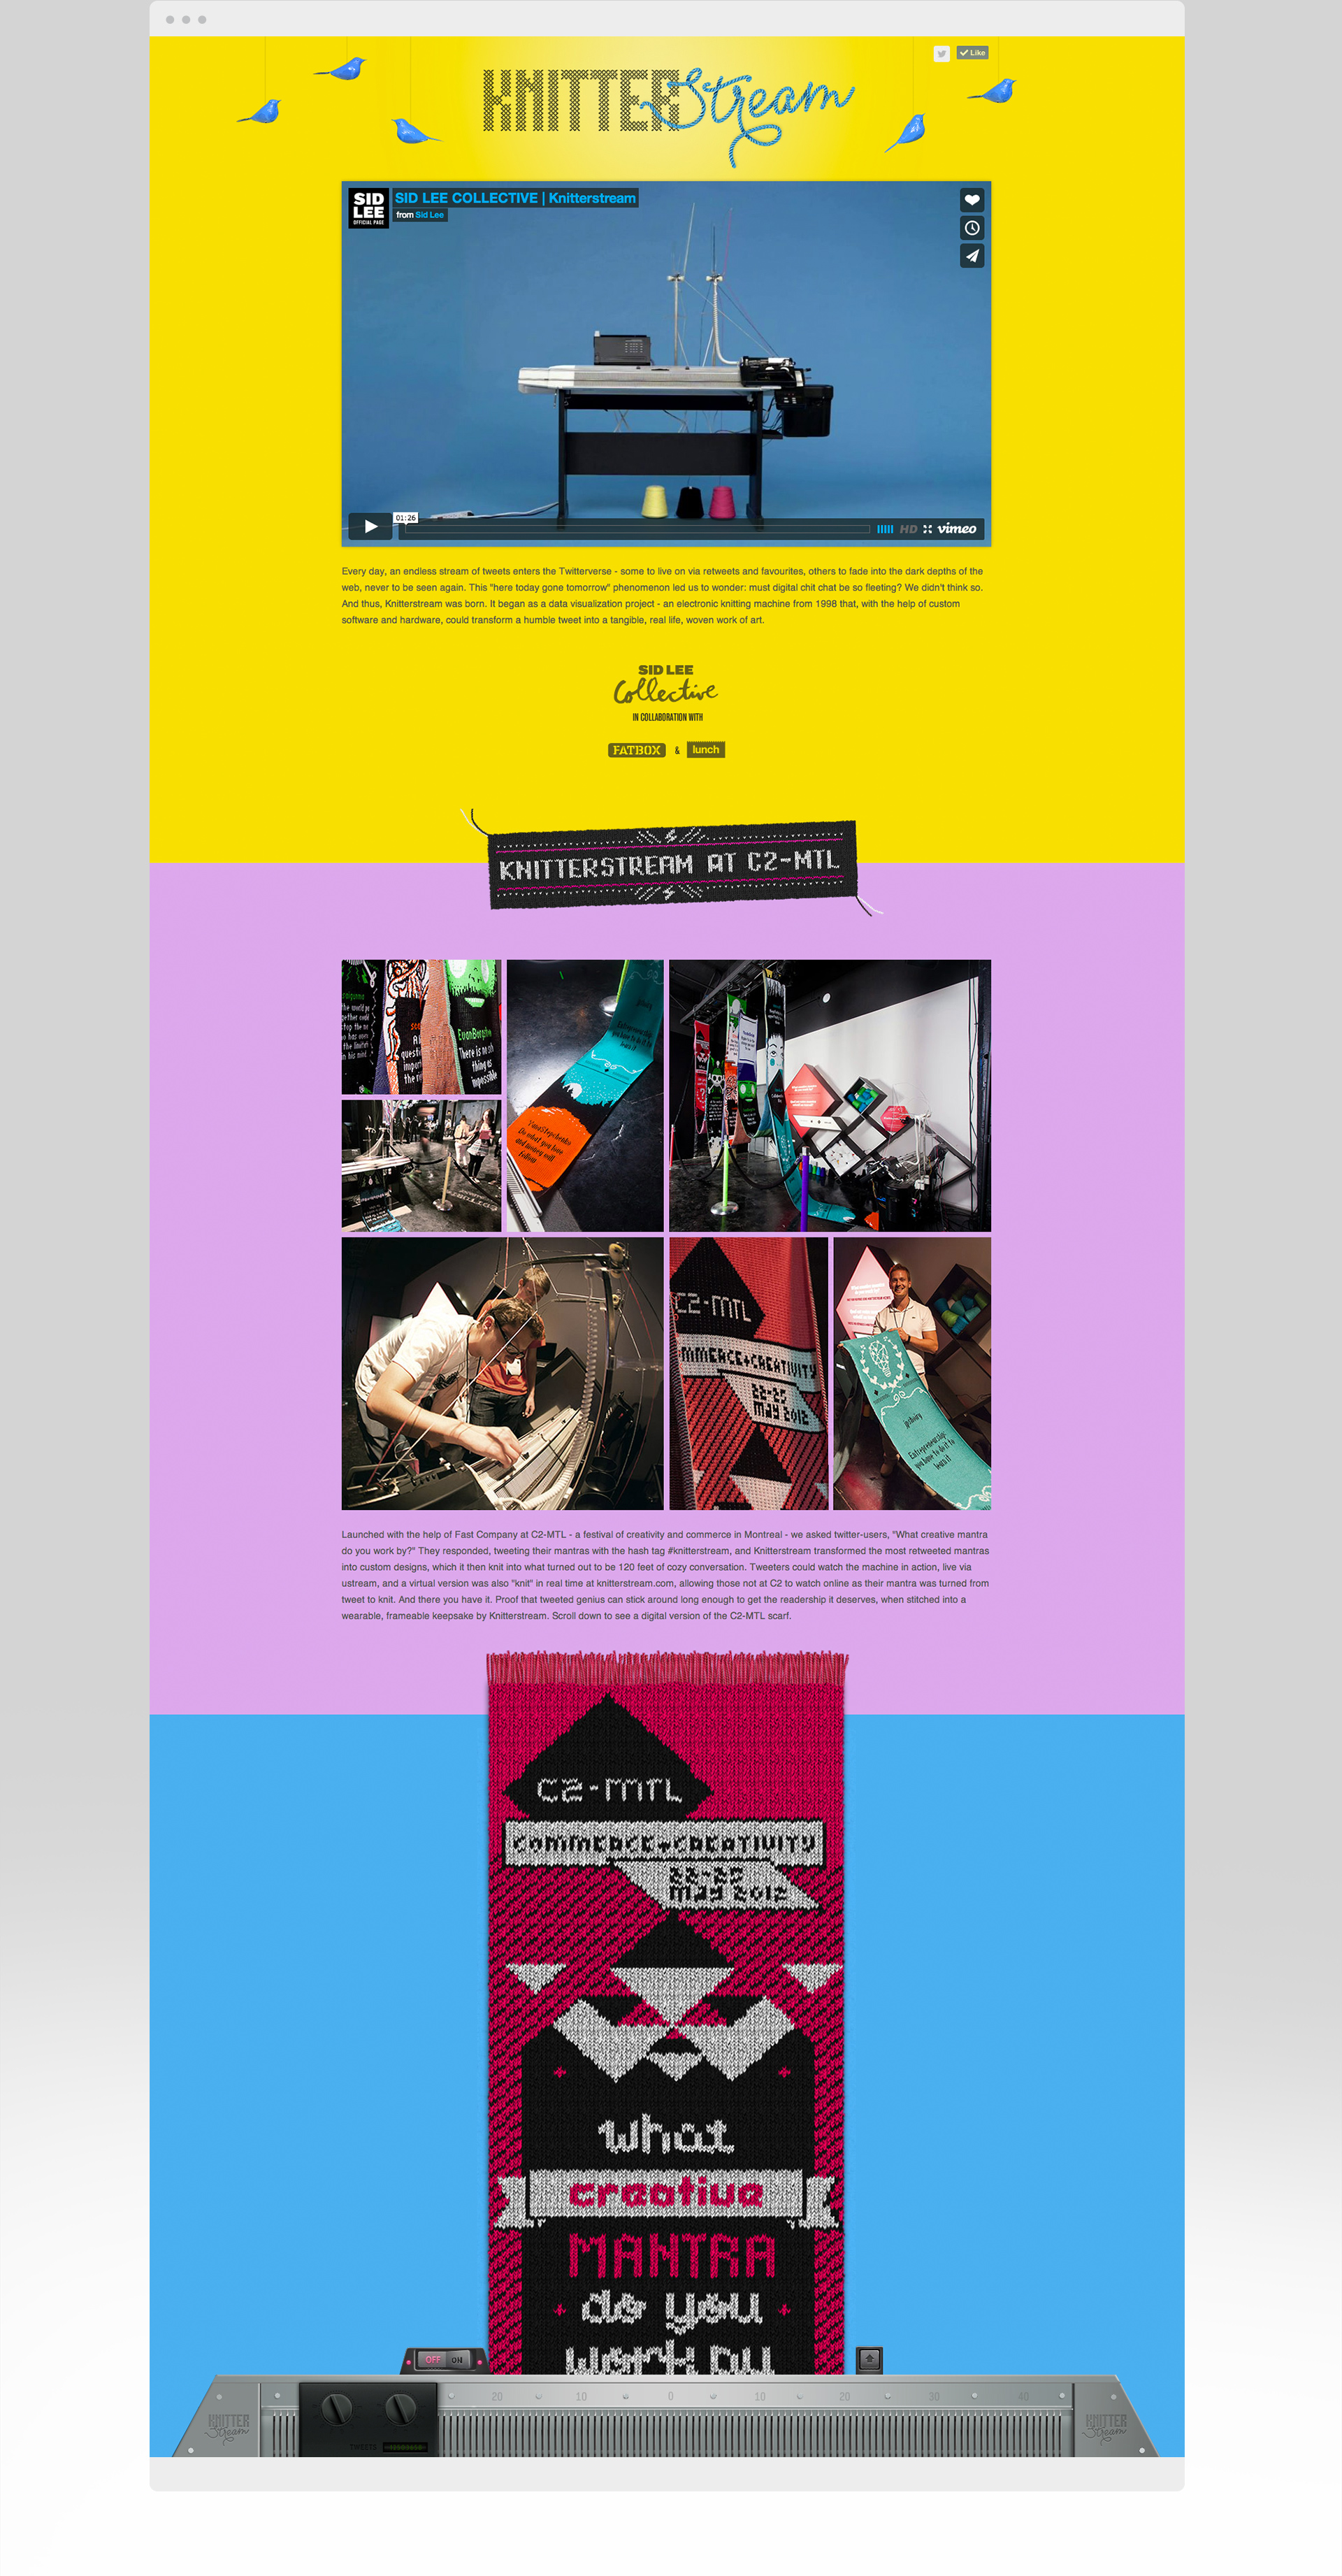
\includegraphics[width=\textwidth, trim={16cm 44cm 16cm 40cm},clip]{include/knitterstream_23.jpg}
        \end{column}

    \end{columns}

\end{frame}

\begin{frame}[allowframebreaks]{Participants}
\begin{columns}
\begin{column}{0.4\linewidth}
    \begin{block}{Instructors}
        \begin{description}
            \item[Hafliði] FABLAB, UI
            \item[Hafsteinn] Computer Science, UI
            \item[Helga] Industrial Eng., UI
            \item[Hörður] Computer \& Electrical Eng., UI
            \item[Ragna] Fashion Design, IUA
        \end{description}
    \end{block}    
\end{column}

\begin{column}{0.45\linewidth}
    \begin{block}{Students}
        \begin{description}
            \item[Elli] Mechanical Eng. and Computer Science, UI.
            \item[Gísa] Fashion Design, IUA.
            \item[Snæja] Applied Mathematics and Computer Science, UI.
        \end{description}
    \end{block}
\end{column}
\end{columns}

\framebreak

\begin{block}{Collaborators}
    \begin{description}
        \item[Icelandic Textile Center] A digital textile workshop in Blöndós, providing spare parts.
        \item[Ístex] Supplies locally sourced yarn.
        \item[The Icelandic Handicraft Association and National Museum of Iceland] Jointly published  \alert{Sjónabók}, which we use as base patterns for our work.
        \item[Marel] A leading manufacturer of equipment for fish processing plants, offering expertise in industrial mechanics and technology.
        \item[\'{Y}rúrarí] \'Yr Jóhannsdóttir, a renowned knitting designer, formerly worked with Passap but now works with \emph{Kniterate}.
        \item[Owen Mace] Retired electrical engineer from South Australia.
    \end{description}
\end{block}

\end{frame}

\begin{frame}{Direction: Machinery}
\centering
\includegraphics[height=0.5\textheight]{include/machines_placeholder.jpg}
\end{frame}

\begin{frame}{Passap Knitting Machines}

% Brief history of Passap
        PASSAP (PAtent Schnell Strick AParat), founded in Switzerland in 1939, was a leader in hobby knitting machines. They ceased production around the turn of the millennium.

% Start the columns environment for comparison
        \begin{columns}

% Left column for Duo 80
            \begin{column}{0.45\textwidth}
                \begin{figure}
                    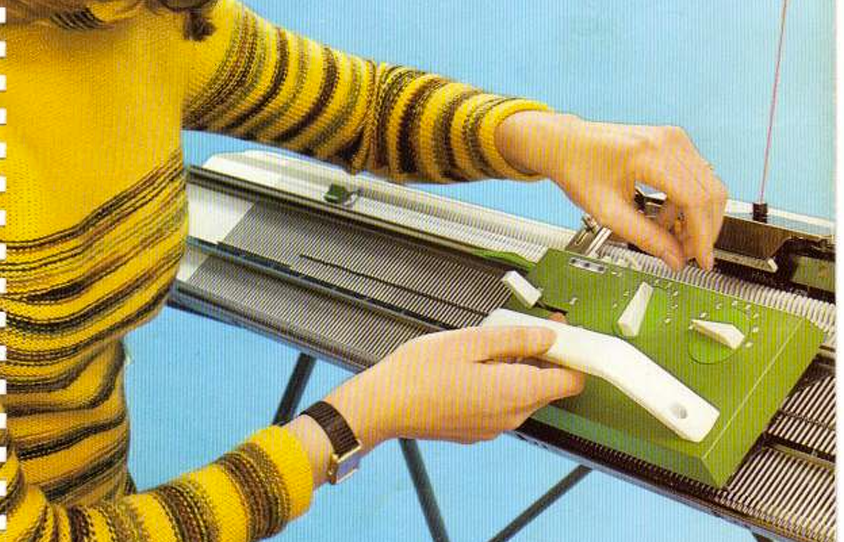
\includegraphics[height=0.3\textheight]{include/duo80.png}
                \end{figure}
                \textbf{Passap Duo 80}
                \begin{itemize}
                    \item \textbf{Motor:} Electra 3000
                    \item \textbf{Color:} Manually switches 4 colors
                    \item \textbf{Pattern:} Simple
                \end{itemize}
            \end{column}

% Right column for E6000
            \begin{column}{0.58\textwidth}
                \begin{figure}
                    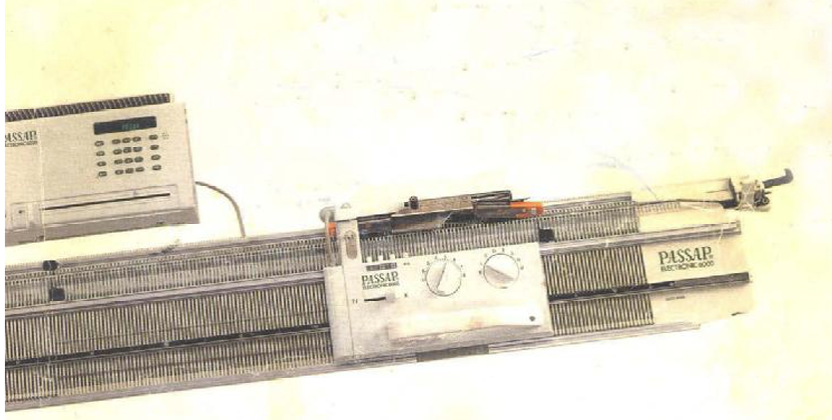
\includegraphics[height=0.3\textheight]{include/e6000.png}
                \end{figure}
                \textbf{Passap E6000}
                \begin{itemize}
                    \item \textbf{Motor:} Electra 4600
                    \item \textbf{Auto Color:} Automatically switches 4 colors
                    \item \textbf{Pattern:} Complex
                \end{itemize}
            \end{column}

        \end{columns}
    \end{frame}

\begin{frame}{Kniterate}

    \href{https://www.kniterate.com/product/kniterate-the-digital-knitting-machine/}{Kniterate}, a digital knitting machine from Spain, designed for small manufacturers. Not intended for mass-production or hobbyists. There are two such machines in Iceland.

    \begin{description}
        \item[Advantage] Originally a ``hack'' of similar 80s/90s knitting machines, it was launched on \href{https://www.kickstarter.com/projects/kniterate/kniterate-the-digital-knitting-machine/}{Kickstarter} in 2017 (then priced at \texteuro{}4,500).
        \item[Disadvantage] Long waiting list and expensive (priced from \texteuro{}16,000).
    \end{description}

    \begin{figure}
        \centering
        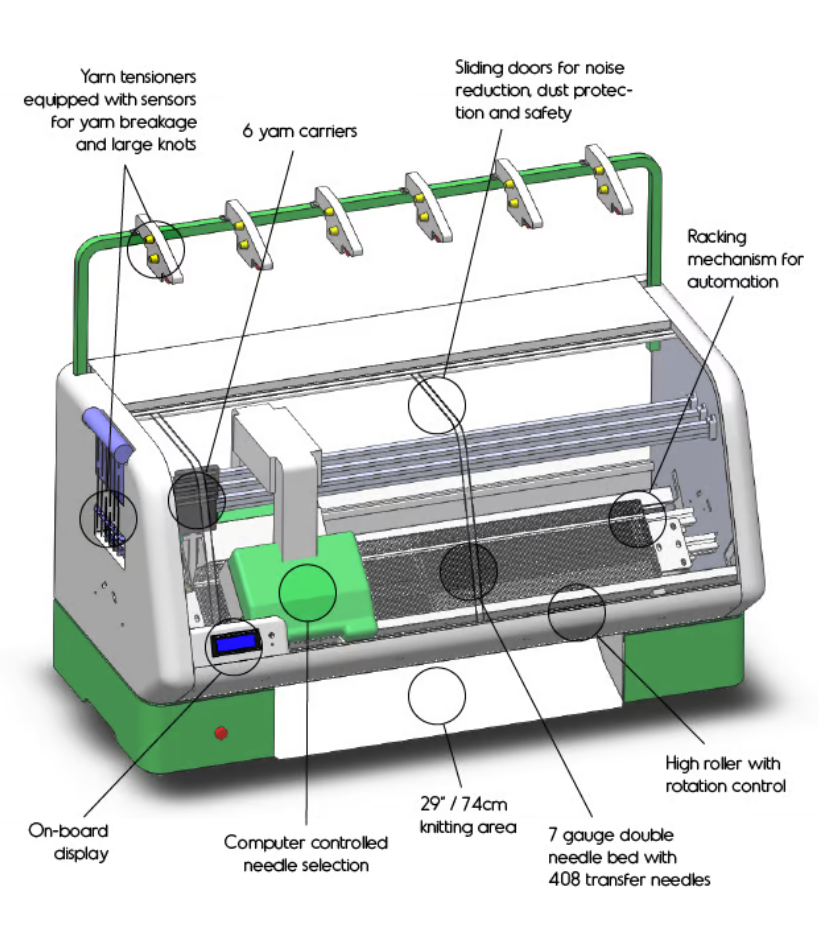
\includegraphics[height=.5\textheight]{include/skema-kniterate.png} ~~~~      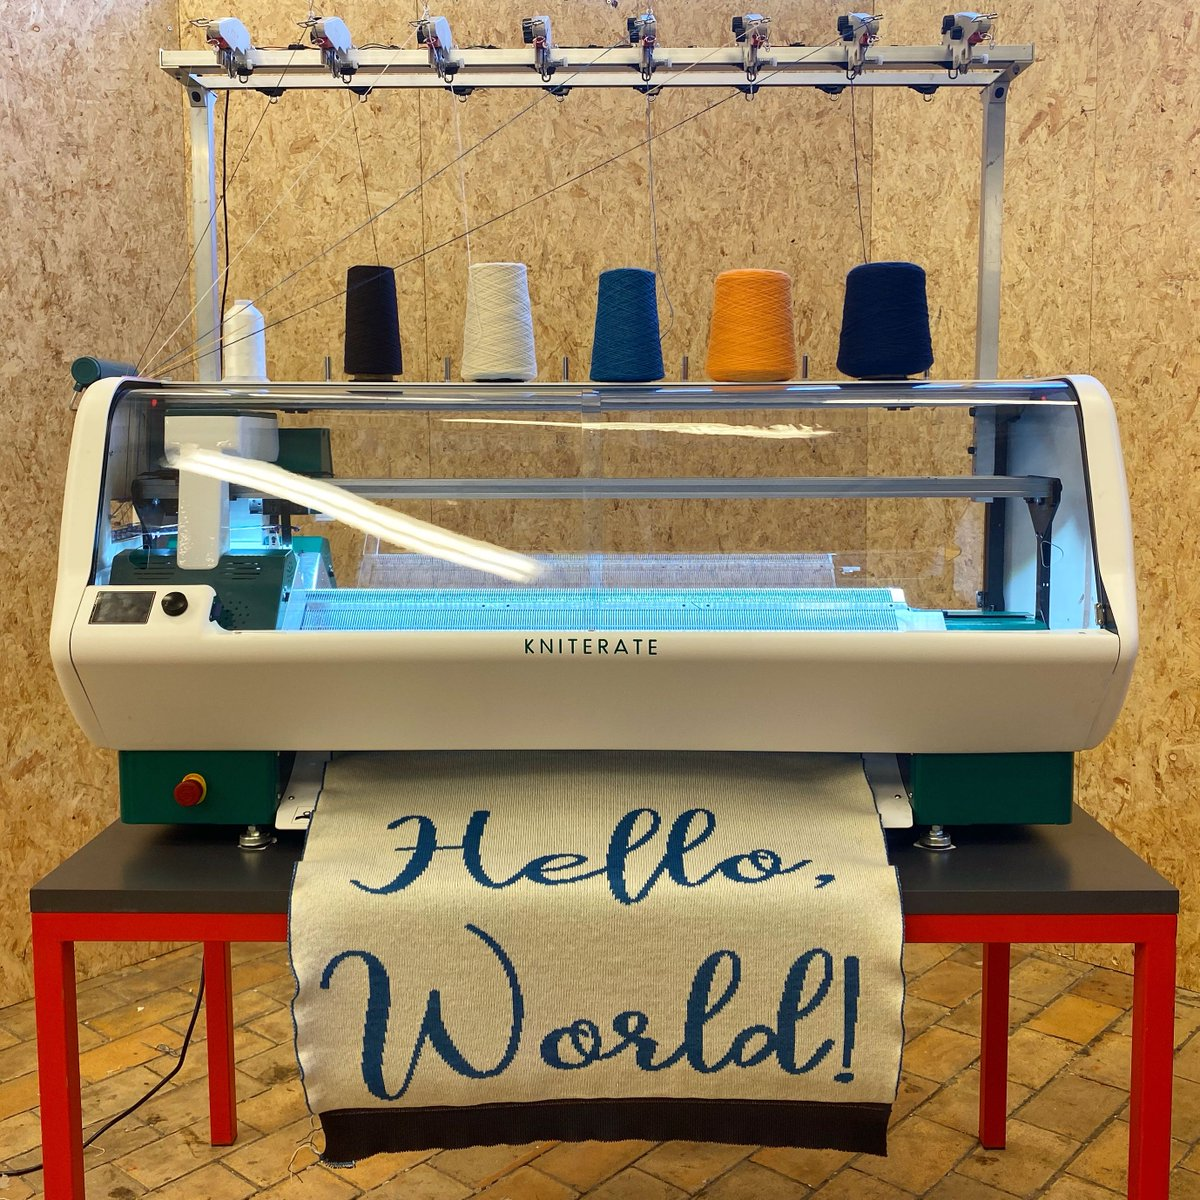
\includegraphics[height=.5\textheight]{include/kniterate-helloworld.jpg}

    \end{figure}
\end{frame}

\begin{frame}{Direction: Knitting Patterns}
\centering
\includegraphics[height=0.5\textheight]{include/sjonabok_placeholder.jpg}
\end{frame}

    \begin{frame}[allowframebreaks]{The Icelandic Sjónabók}

        \begin{columns}
            \begin{column}{0.7\textwidth}
                \begin{block}{What is Sjónabók?}
                    It is a culturally significant collection of traditional Icelandic patterns used in various handcrafted items throughout Icelandic history. This manuscript includes patterns from the 16\textsuperscript{th}, 17\textsuperscript{th}, and 18\textsuperscript{th} centuries. Published in 2009, it contains 10 preserved manuscripts and is unfortunately out of print.
                \end{block}

                \begin{itemize}
                    \item \textbf{Translation:} The term ``Sjónabók'' can be translated as ``Book of Visual Patterns.''
                    \item \textbf{Content:} Contains patterns and motifs used in textiles, with text in both Icelandic and English.
                \end{itemize}
            \end{column}

            \begin{column}{0.3\textwidth}
                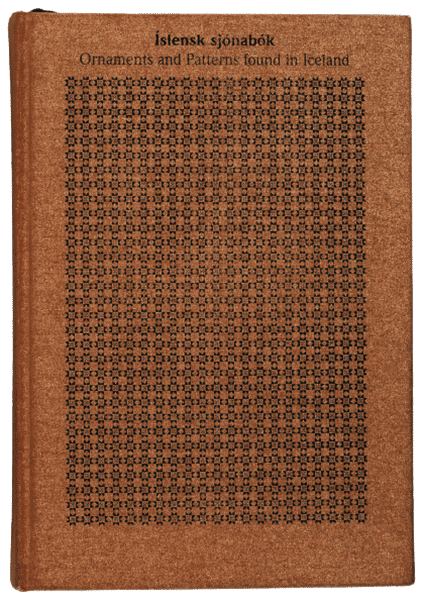
\includegraphics[width=\textwidth]{include/sjónabók.png}
            \end{column}
        \end{columns}

        \framebreak

        \begin{figure}
            \centering
            \caption{Manuscript at the Icelandic National Museum}
            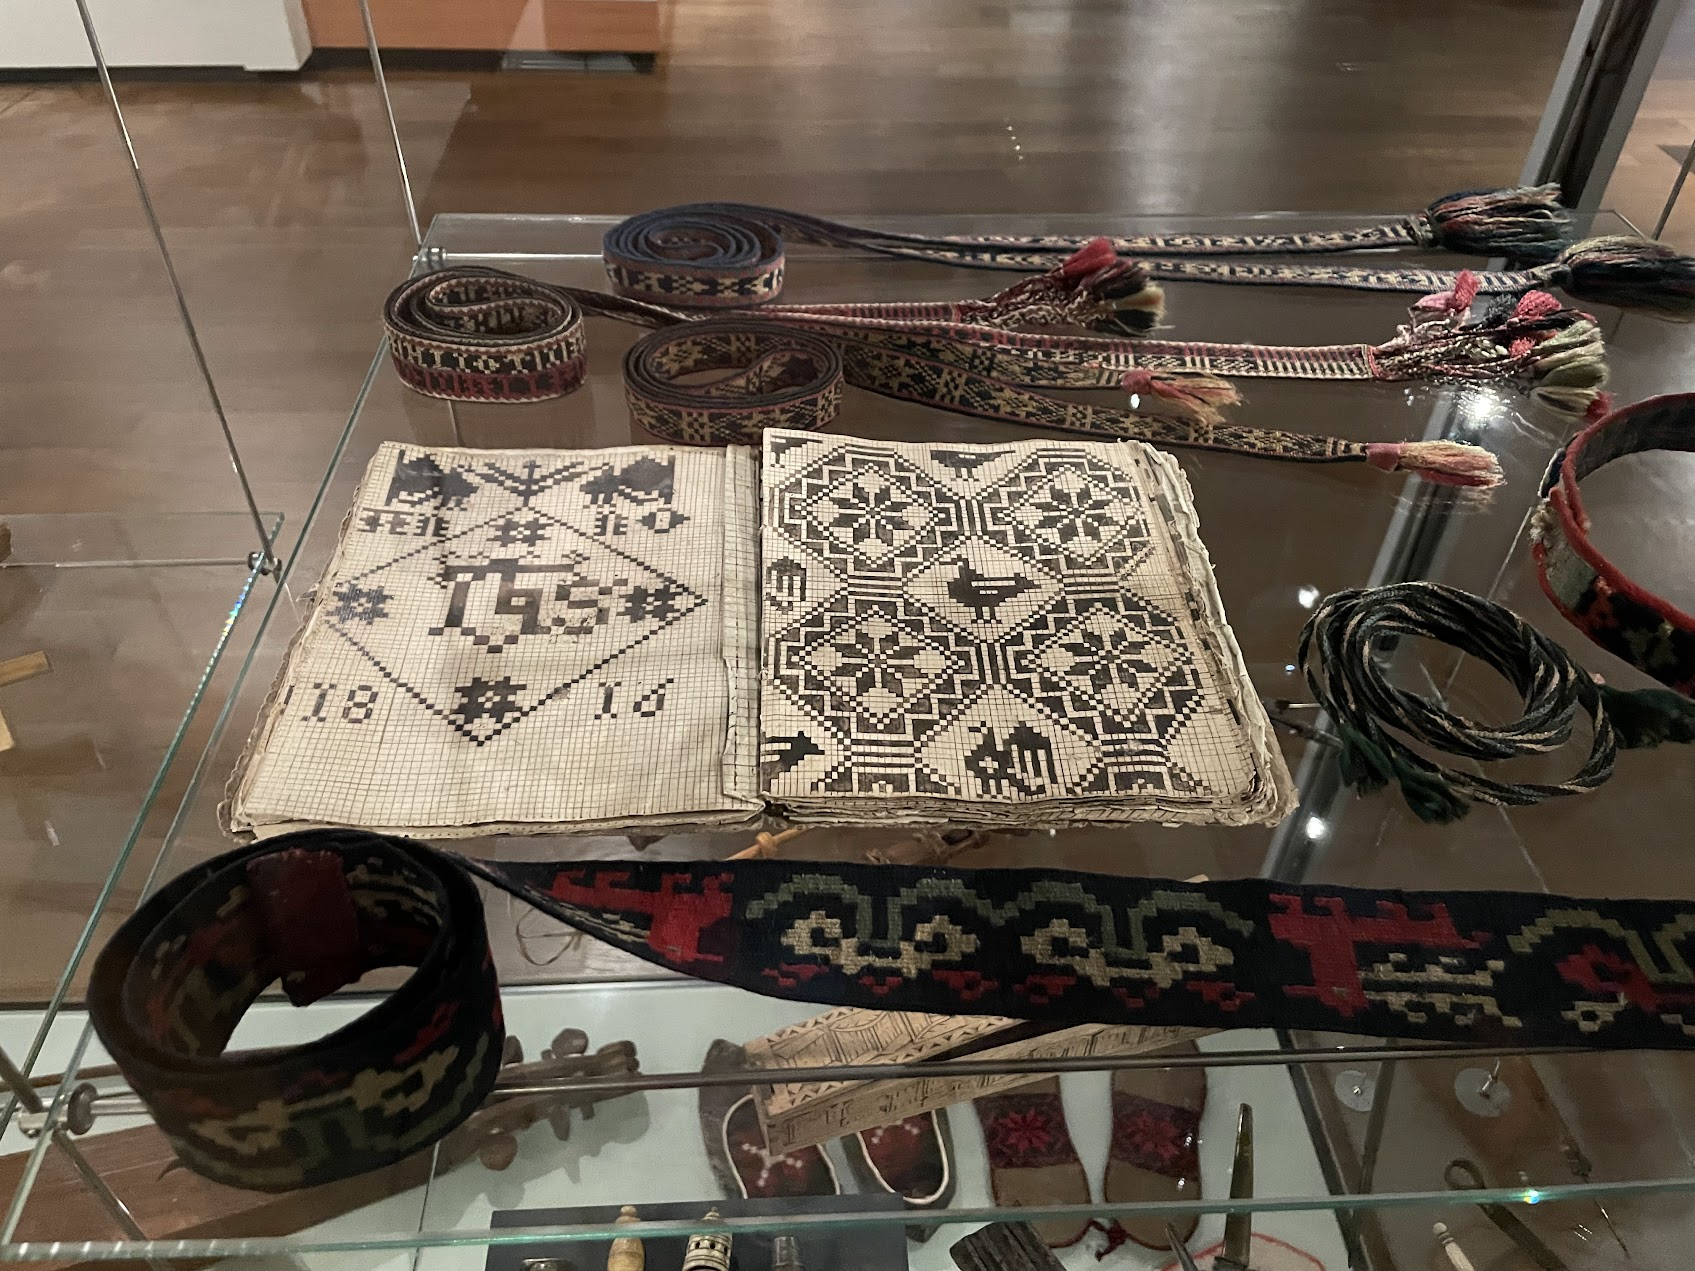
\includegraphics[width=0.49\textwidth]{include/sjónabók-safn.jpg}
            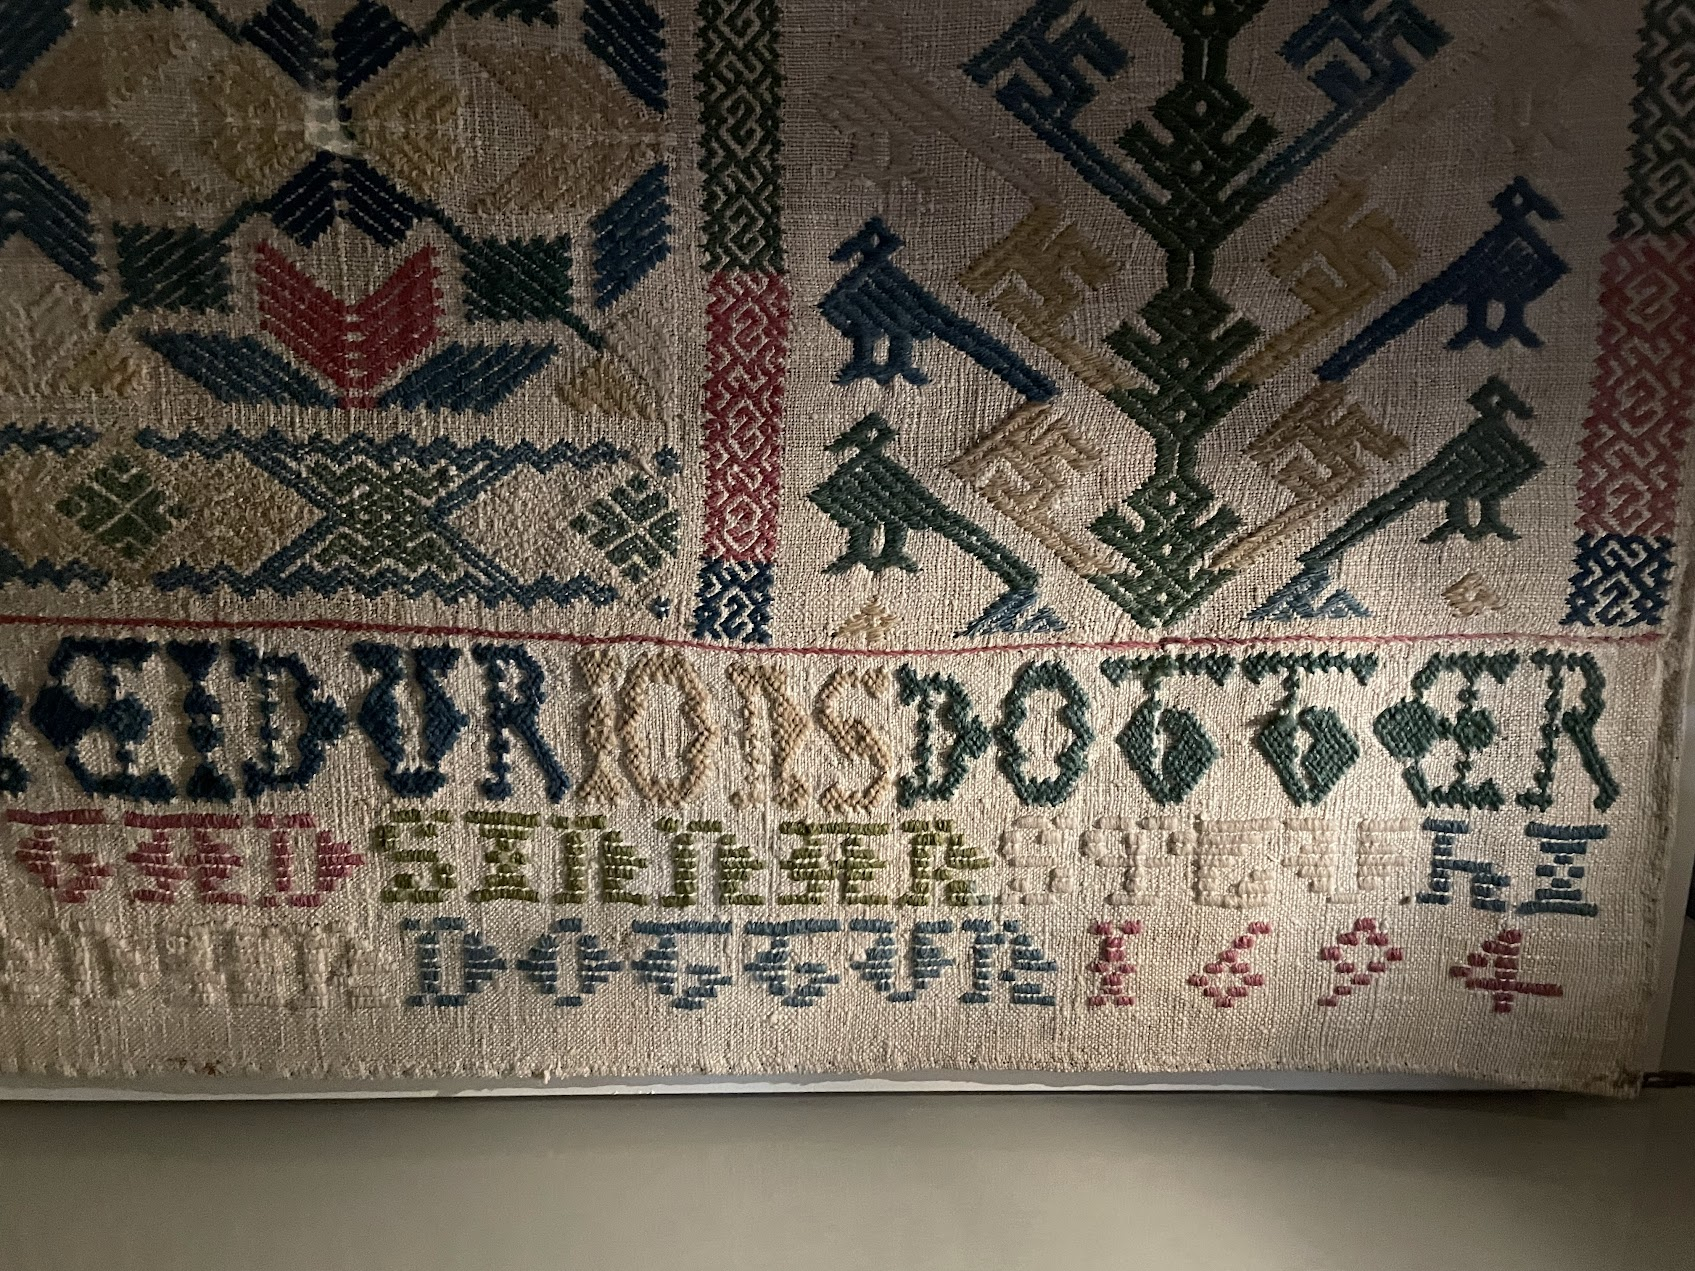
\includegraphics[width=0.49\textwidth]{include/jonsdottir.jpg}

            \framebreak

            \caption{Passage from Hallgrímur Pétursson's  \textit{Passion Hymns}}
            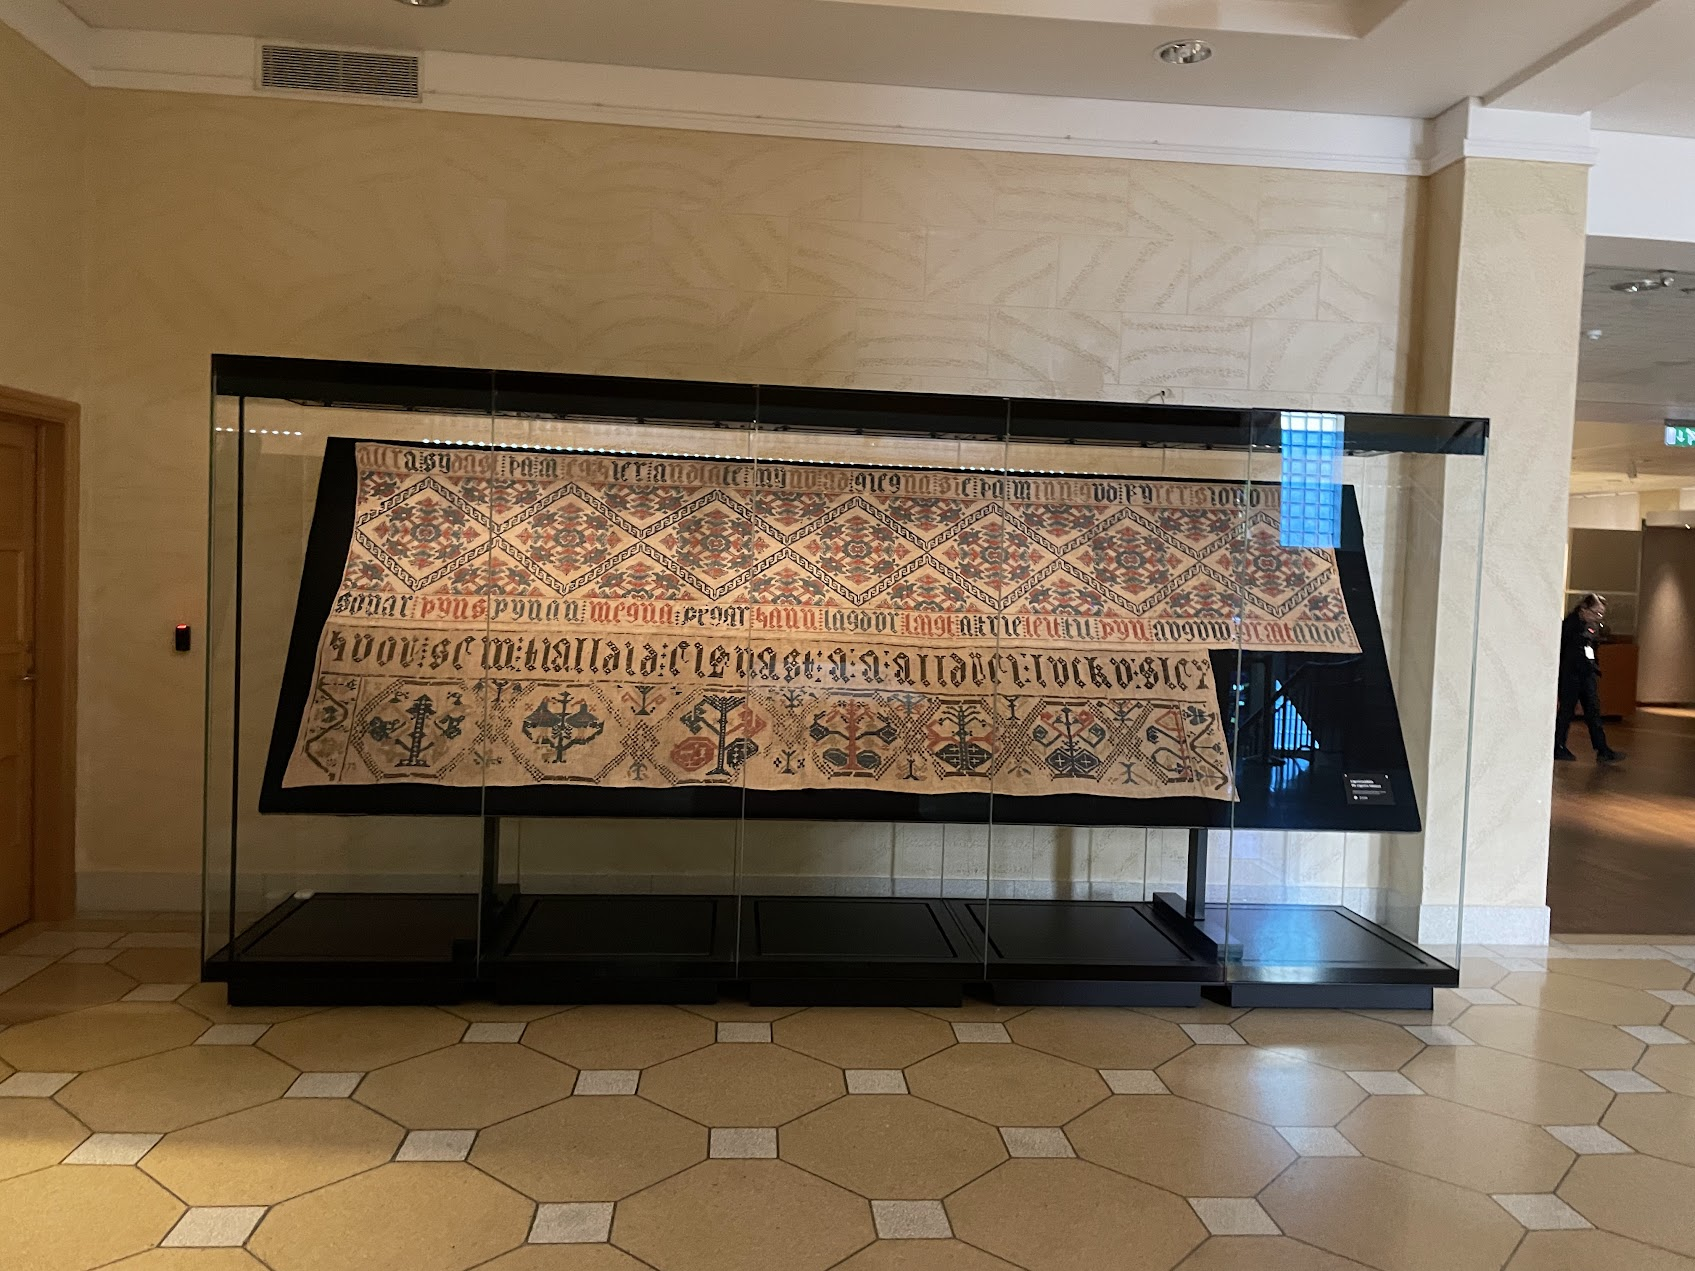
\includegraphics[width=0.49\textwidth]{include/passiusalmur.jpg}
            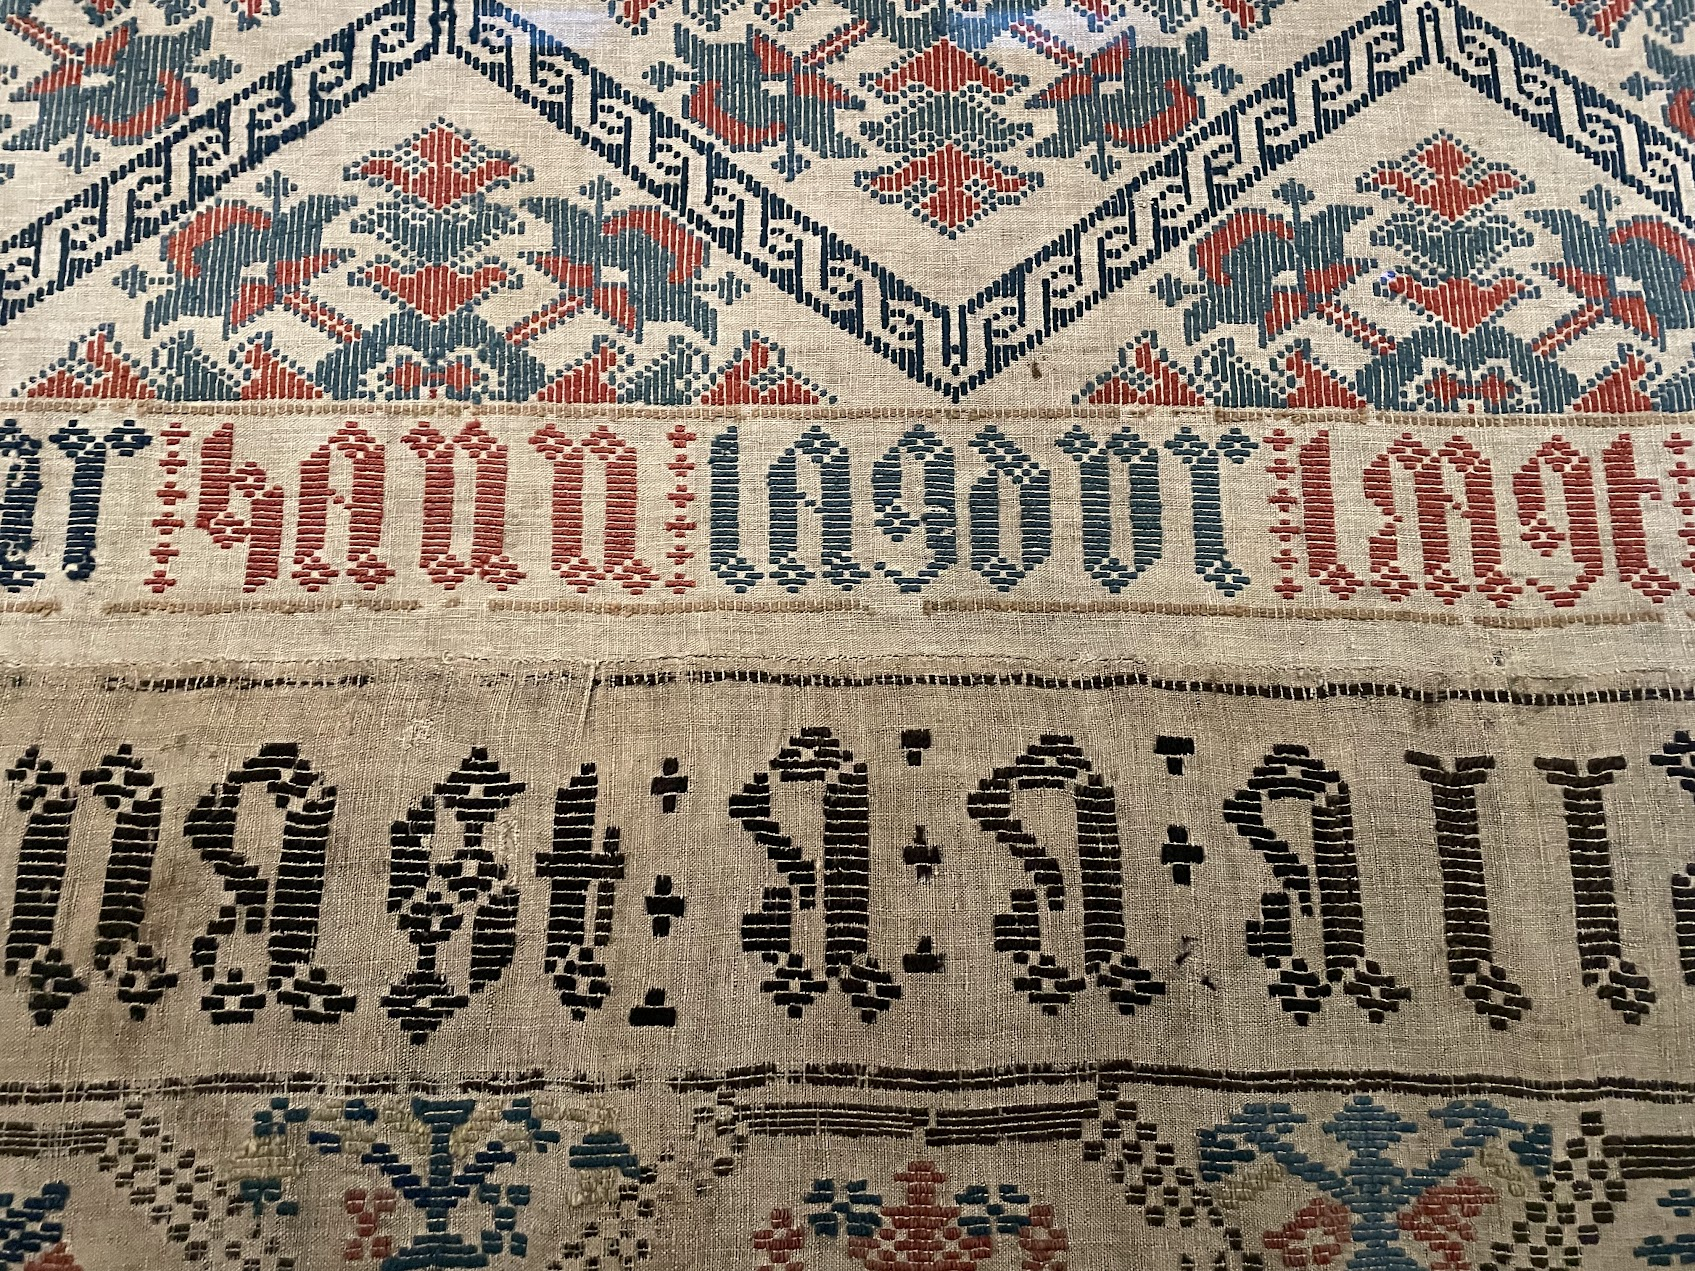
\includegraphics[width=0.49\textwidth]{include/passiusalmur-zoom.jpg}


            \framebreak
            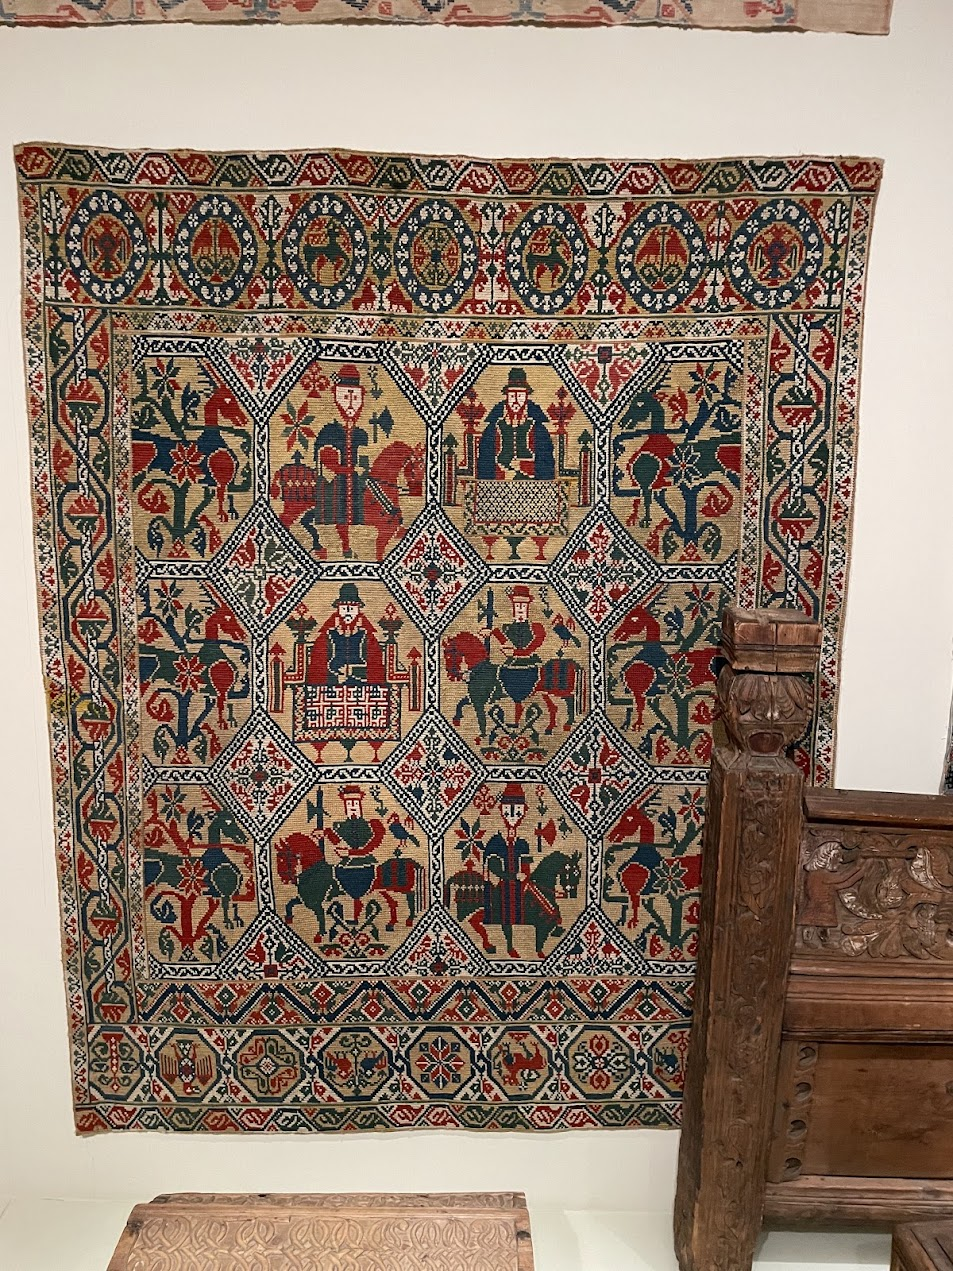
\includegraphics[width=0.3\textwidth]{include/riddarateppi.jpg}
            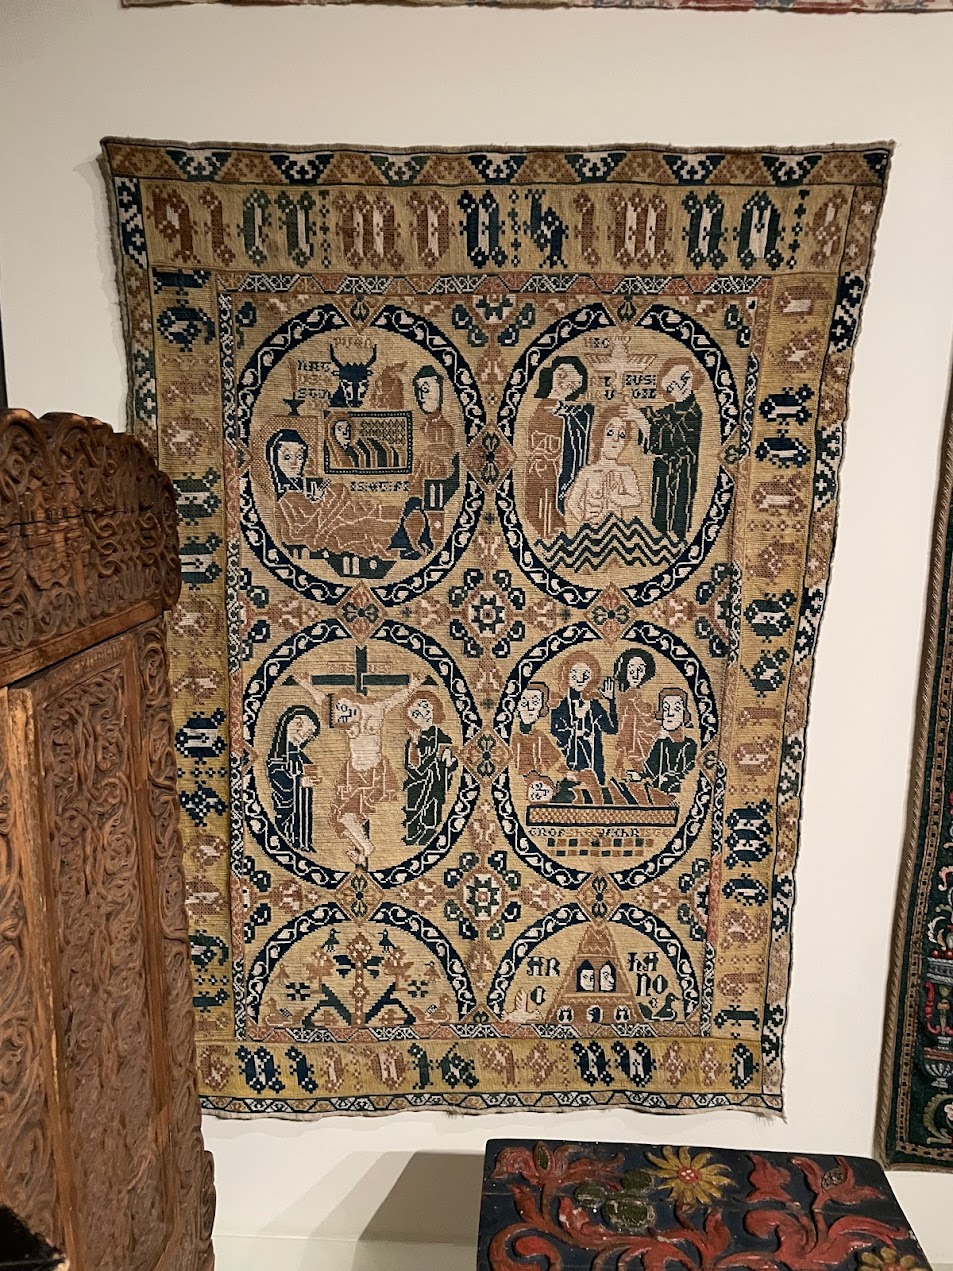
\includegraphics[width=0.3\textwidth]{include/ævijesú.jpg}
        \end{figure}

        \framebreak

        \begin{figure}

            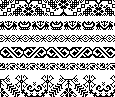
\includegraphics[height=.65\textheight]{include/thjms2008-14_560.png}\hspace{24pt}
            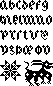
\includegraphics[height=.65\textheight]{include/thjms2008-14_562.png}
        \end{figure}
        \url{https://github.com/HiDefTextiles/Sjonabok}
    \end{frame}


\begin{frame}{Direction: Knitting Swatches}
\centering
\includegraphics[height=0.5\textheight]{include/knits_placeholder.jpg}
\end{frame}

    \begin{frame}{Hello World}
        \begin{figure}
            \centering
            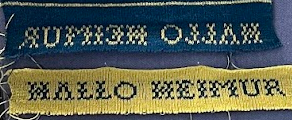
\includegraphics[height=36pt, clip=true, trim=0 5mm 0 0]{include/helloworld.png}
            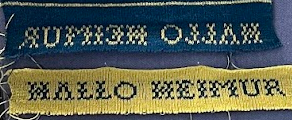
\includegraphics[height=36pt, clip=true, trim=0 0 0 5mm]{include/helloworld.png}
        \end{figure}


        \begin{itemize}
            \item \textbf{Introduction to Programming:} "Hello World" is often the first program written by beginners in computer science.
            \item \textbf{Significance:} Demonstrates the basic structure of a program, outputting text to the screen.
            \item \textbf{Tradition:} Used as a rite of passage for learning a new programming language or environment.
        \end{itemize}
    \end{frame}

    \begin{frame}{Icelandic Peacock}
        \centering
        \href{https://www.instagram.com/p/C9Cf8FFgDZZ/}{
            
\includegraphics[height=.7\textheight]{include/thjms5898_246_0.png}
            \hspace{24pt}
            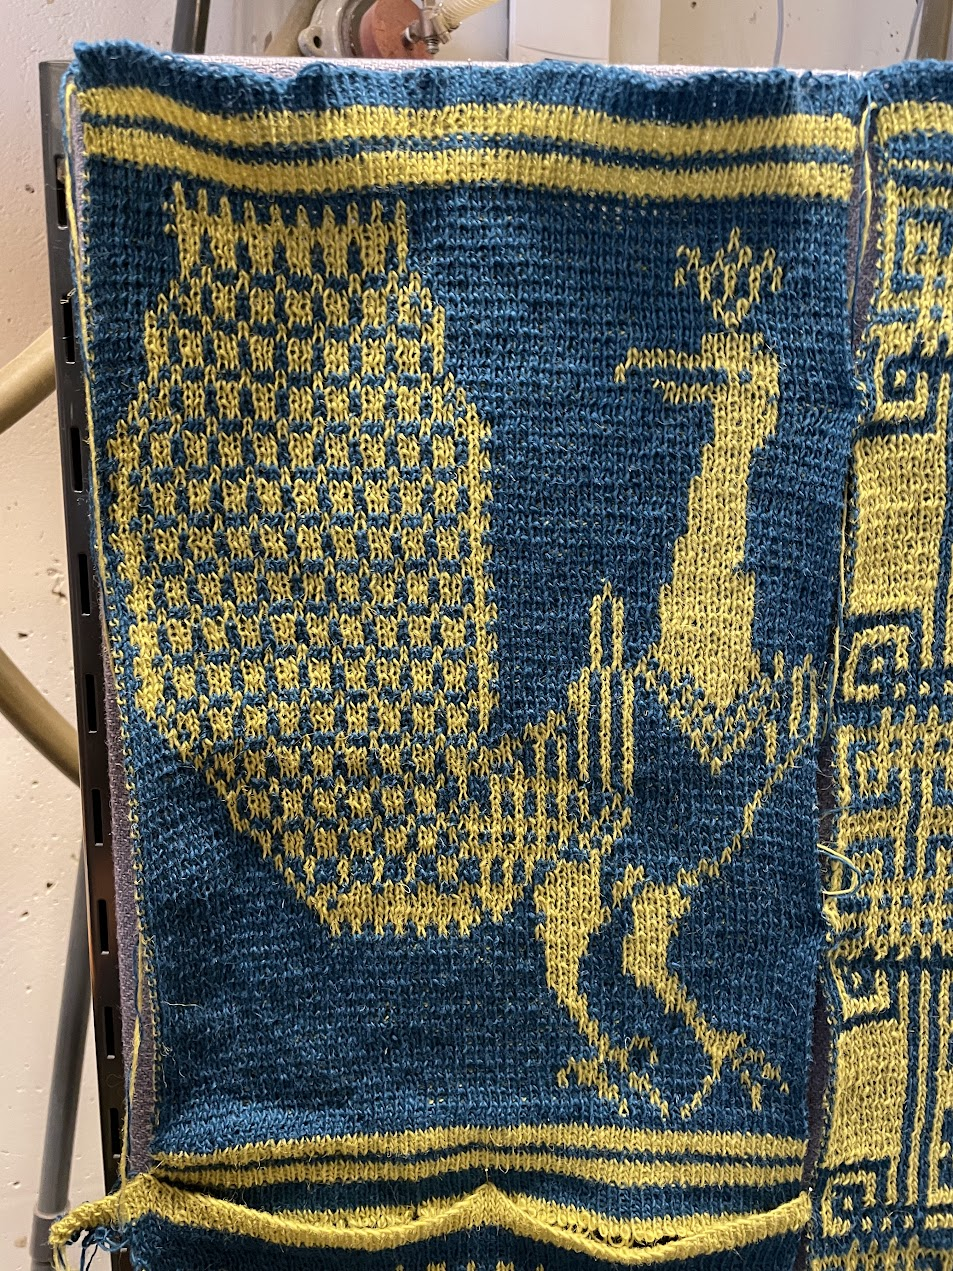
\includegraphics[height=.7\textheight]{include/peacock.jpg}}
    \end{frame}

    \begin{frame}{Icelandic Flower}
        \centering
        
\includegraphics[height=.7\textheight]{include/thjms5898_210.png}
        \hspace{24pt}
        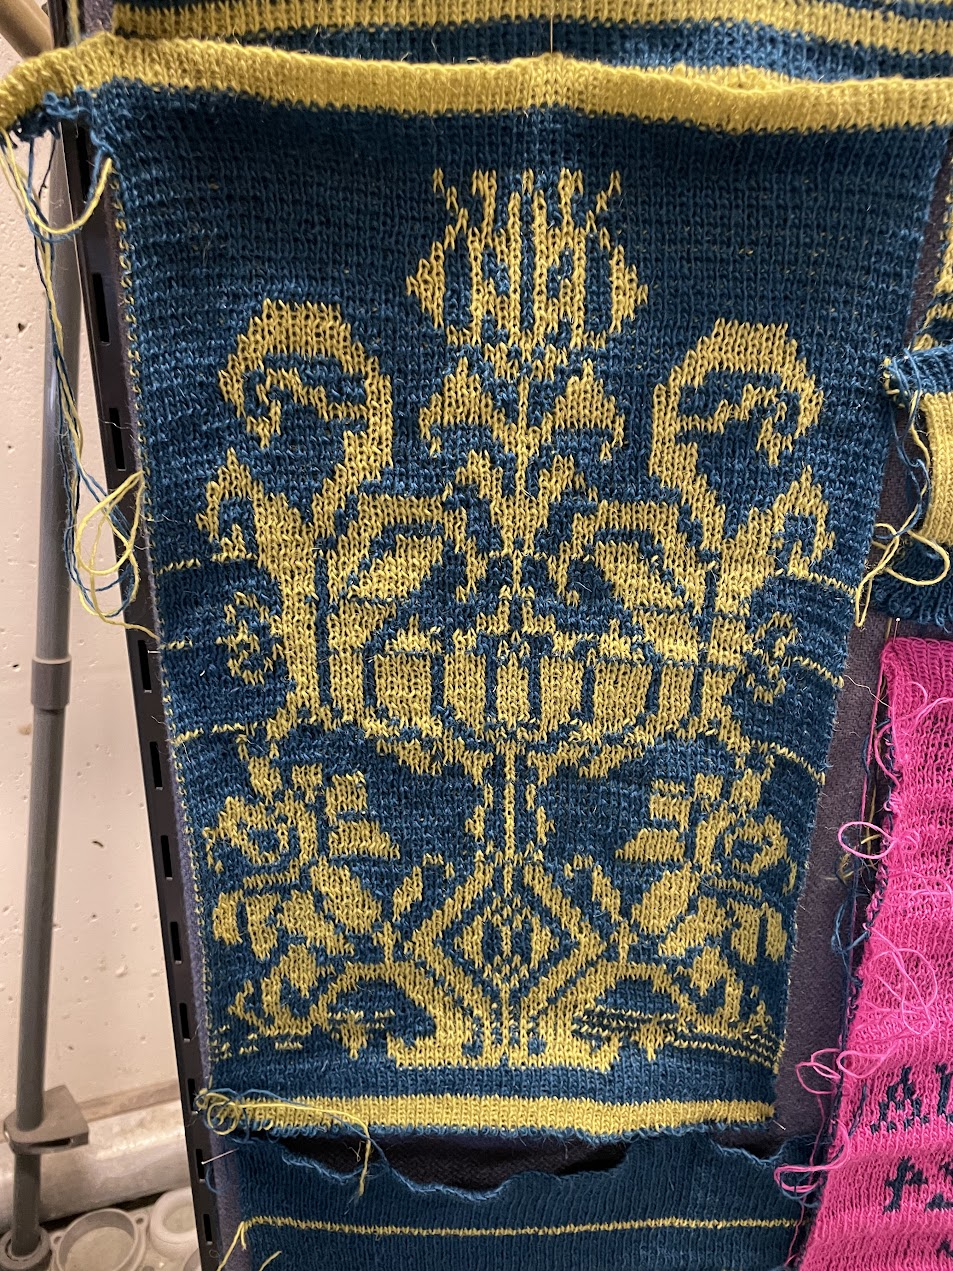
\includegraphics[height=.7\textheight]{include/flower.jpg}
    \end{frame}

    \begin{frame}{Repeated Motif}
        \centering
        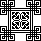
\includegraphics[height=.7\textheight]{include/thjms5898_268.png}
        \hspace{24pt}
        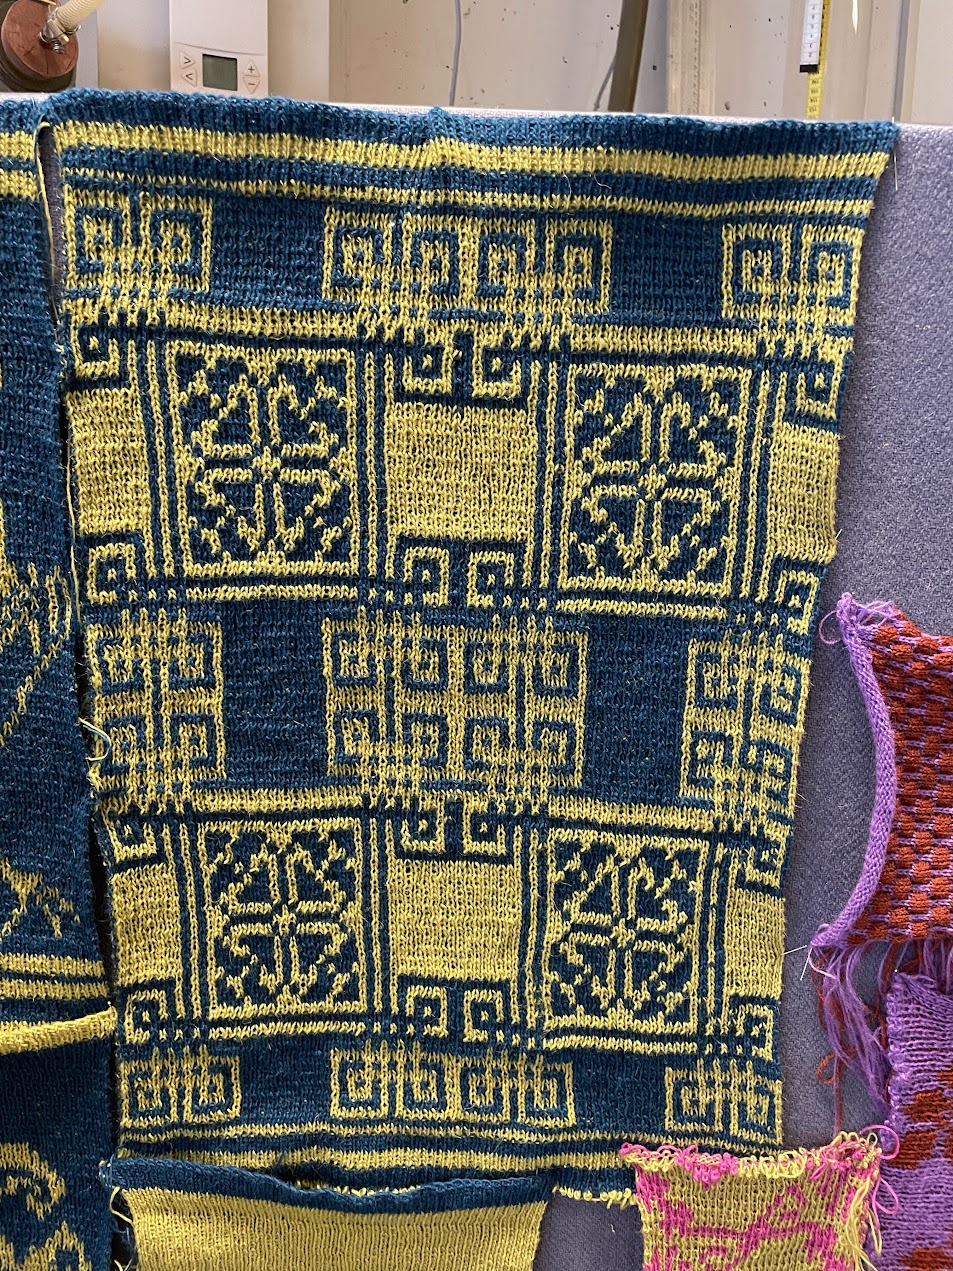
\includegraphics[height=.7\textheight]{include/repeat.jpg}
    \end{frame}


    \begin{frame}{Pets}
        \centering
        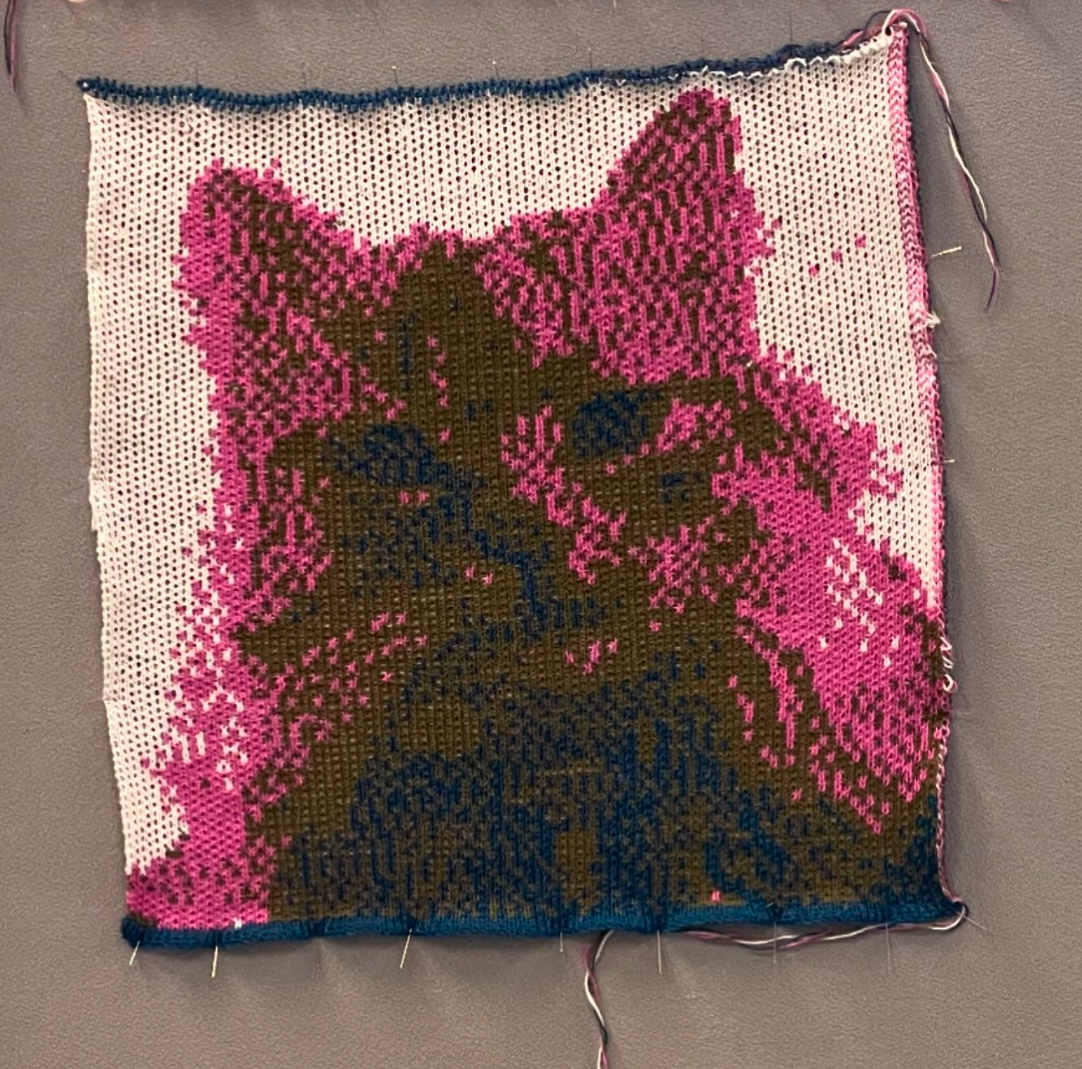
\includegraphics[height=.7\textheight]{include/kisa.png}
        \hspace{24pt}
        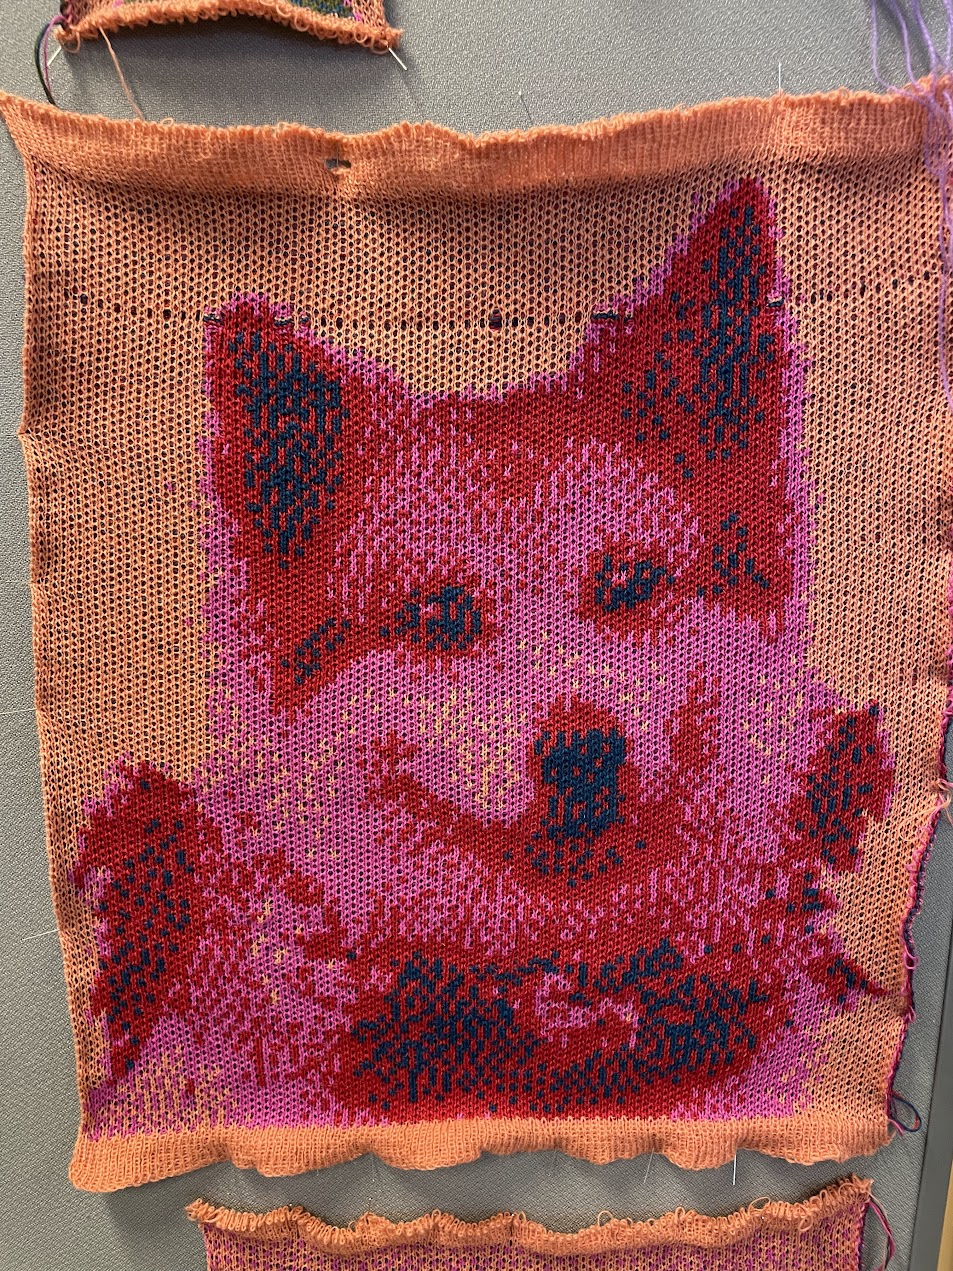
\includegraphics[height=.7\textheight]{include/hundur.jpg}

    \end{frame}


    \begin{frame}{Ragnheiður Jónsdóttir (1646-1715)}
        \begin{columns}
            \begin{column}{.5\linewidth}
                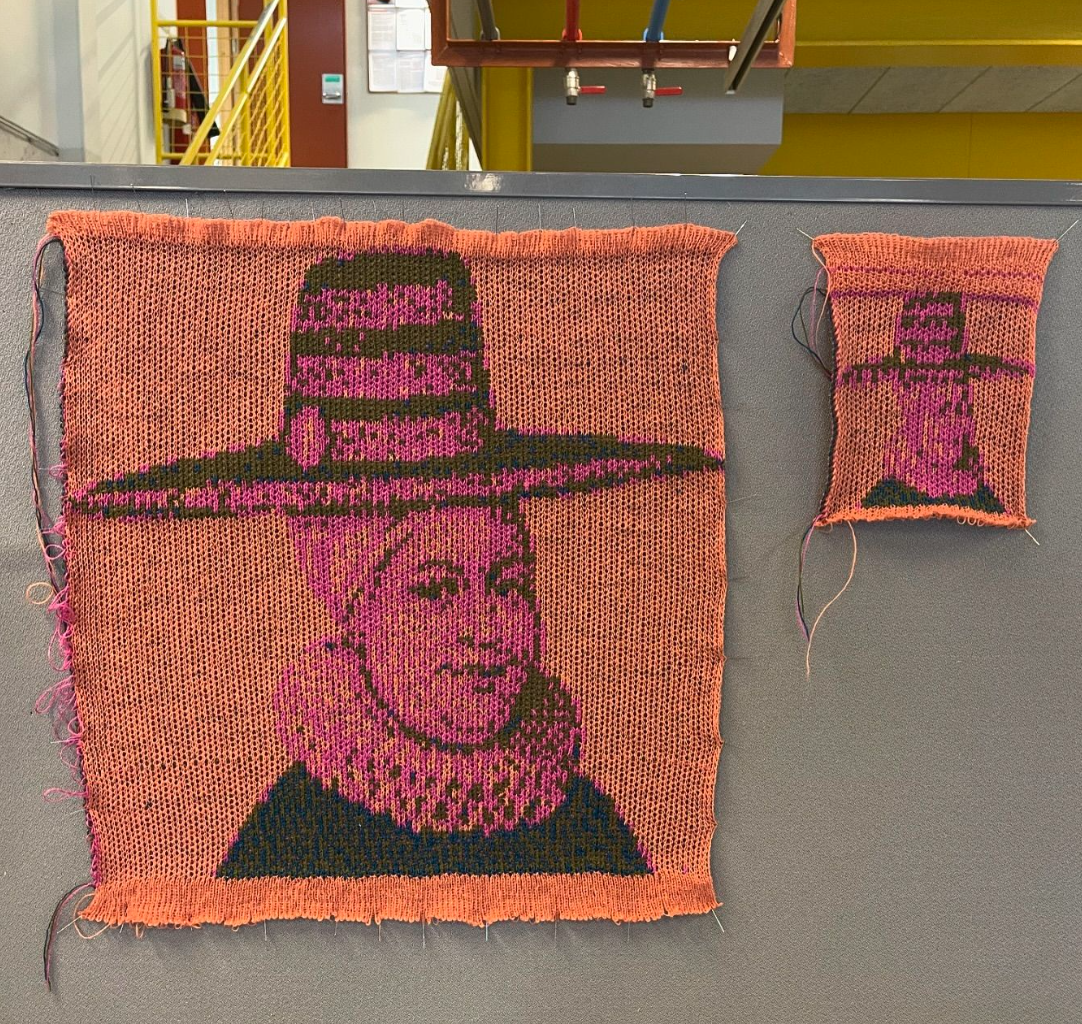
\includegraphics[width=\linewidth]{include/ragnheidur.png}
            \end{column}
            \begin{column}{.5\linewidth}
                \begin{block}{Bishop's Wife}
                    Ragnheiður was a patron of the arts and crafts and played a pivotal role in preserving traditional Icelandic patterns.

                    Her legacy is immortalized on the 5,000 króna banknote
                \end{block}
                \centering
                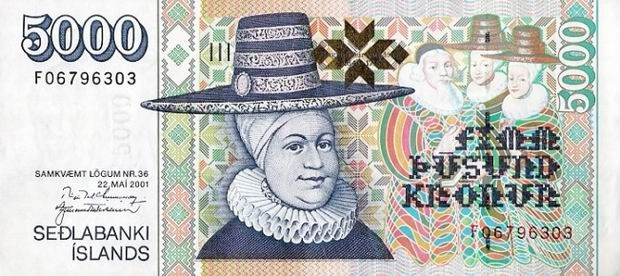
\includegraphics[width=.7\linewidth]{include/5000kr.JPG}
            \end{column}
        \end{columns}
    \end{frame}


    \begin{frame}{Brynjólfur Sveinsson (1605–1675)}
        \begin{columns}
            \begin{column}{.65\linewidth}
                \begin{block}{Bishop of Skálholt}
                    Brynjólfur was the Lutheran Bishop, renowned for his efforts in preserving Icelandic literary heritage. He contributed to the collection of Old Norse manuscripts, including \emph{Book of Flatey}, and played a key role in naming the \emph{Edda} collection.

                    He is honored on the 1,000 króna banknote.
                \end{block}
                \centering
                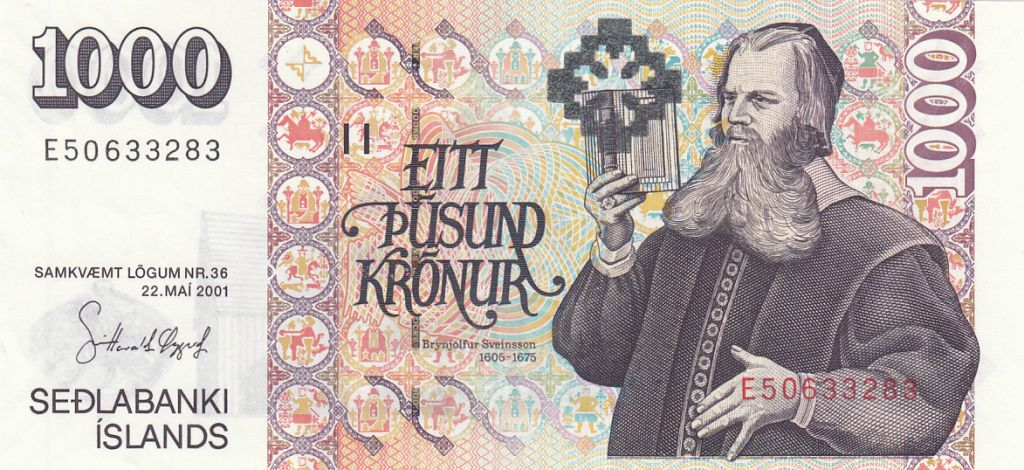
\includegraphics[width=.5\linewidth]{include/1000kr.JPG}
            \end{column}
            \begin{column}{.35\linewidth}
                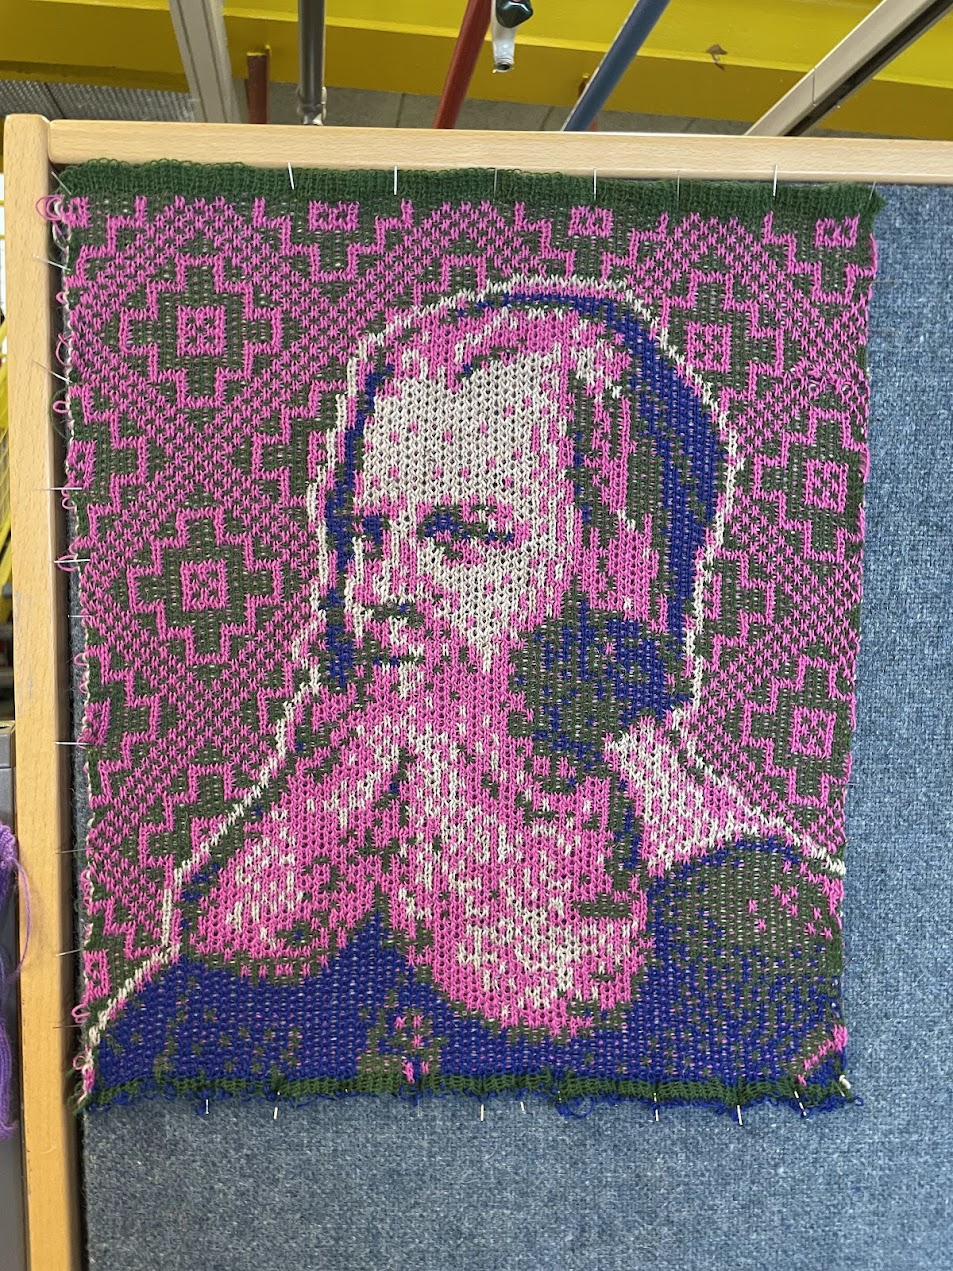
\includegraphics[height=.75\textheight]{include/sveinsson.jpg}
            \end{column}


        \end{columns}

\end{frame}

\begin{frame}{Direction: What Next?}
\centering
\includegraphics[height=0.5\textheight]{include/future_placeholder.jpg}
\end{frame}


\begin{frame}{Lessons Learned and Next Steps}
    \begin{itemize}
        \item \textbf{Hardware Improvements:} While the machine is functional, there are kinks in hardware control, especially in color changes, requiring upgrades.
        \item \textbf{Pattern Workflow:} Experimentation with generative AI superimposed with \emph{Sjónabók} patterns shows promise, but the workflow needs further refinement.
        \item \textbf{Future Vision:} Hardware upgrades to make the more common Duo 80 model as capable as the E6000 would be a significant advancement.
    \end{itemize}
\end{frame}

\begin{frame}{Where Can You See the Machine in Action?}
\begin{columns}
\begin{column}{0.6\linewidth}
    \begin{itemize}
        \item \textbf{September 2024:} Showcased at \alert{Vísindavaka Rannís}.
        \item \textbf{February 2025:} Will appear at \alert{UTmessan}.
        \item \textbf{April 2026:} Planned for \alert{Design March} and a residency at \alert{The Museum of Design and Applied Art}.
    \end{itemize}
\end{column}
\begin{column}{0.4\linewidth}
    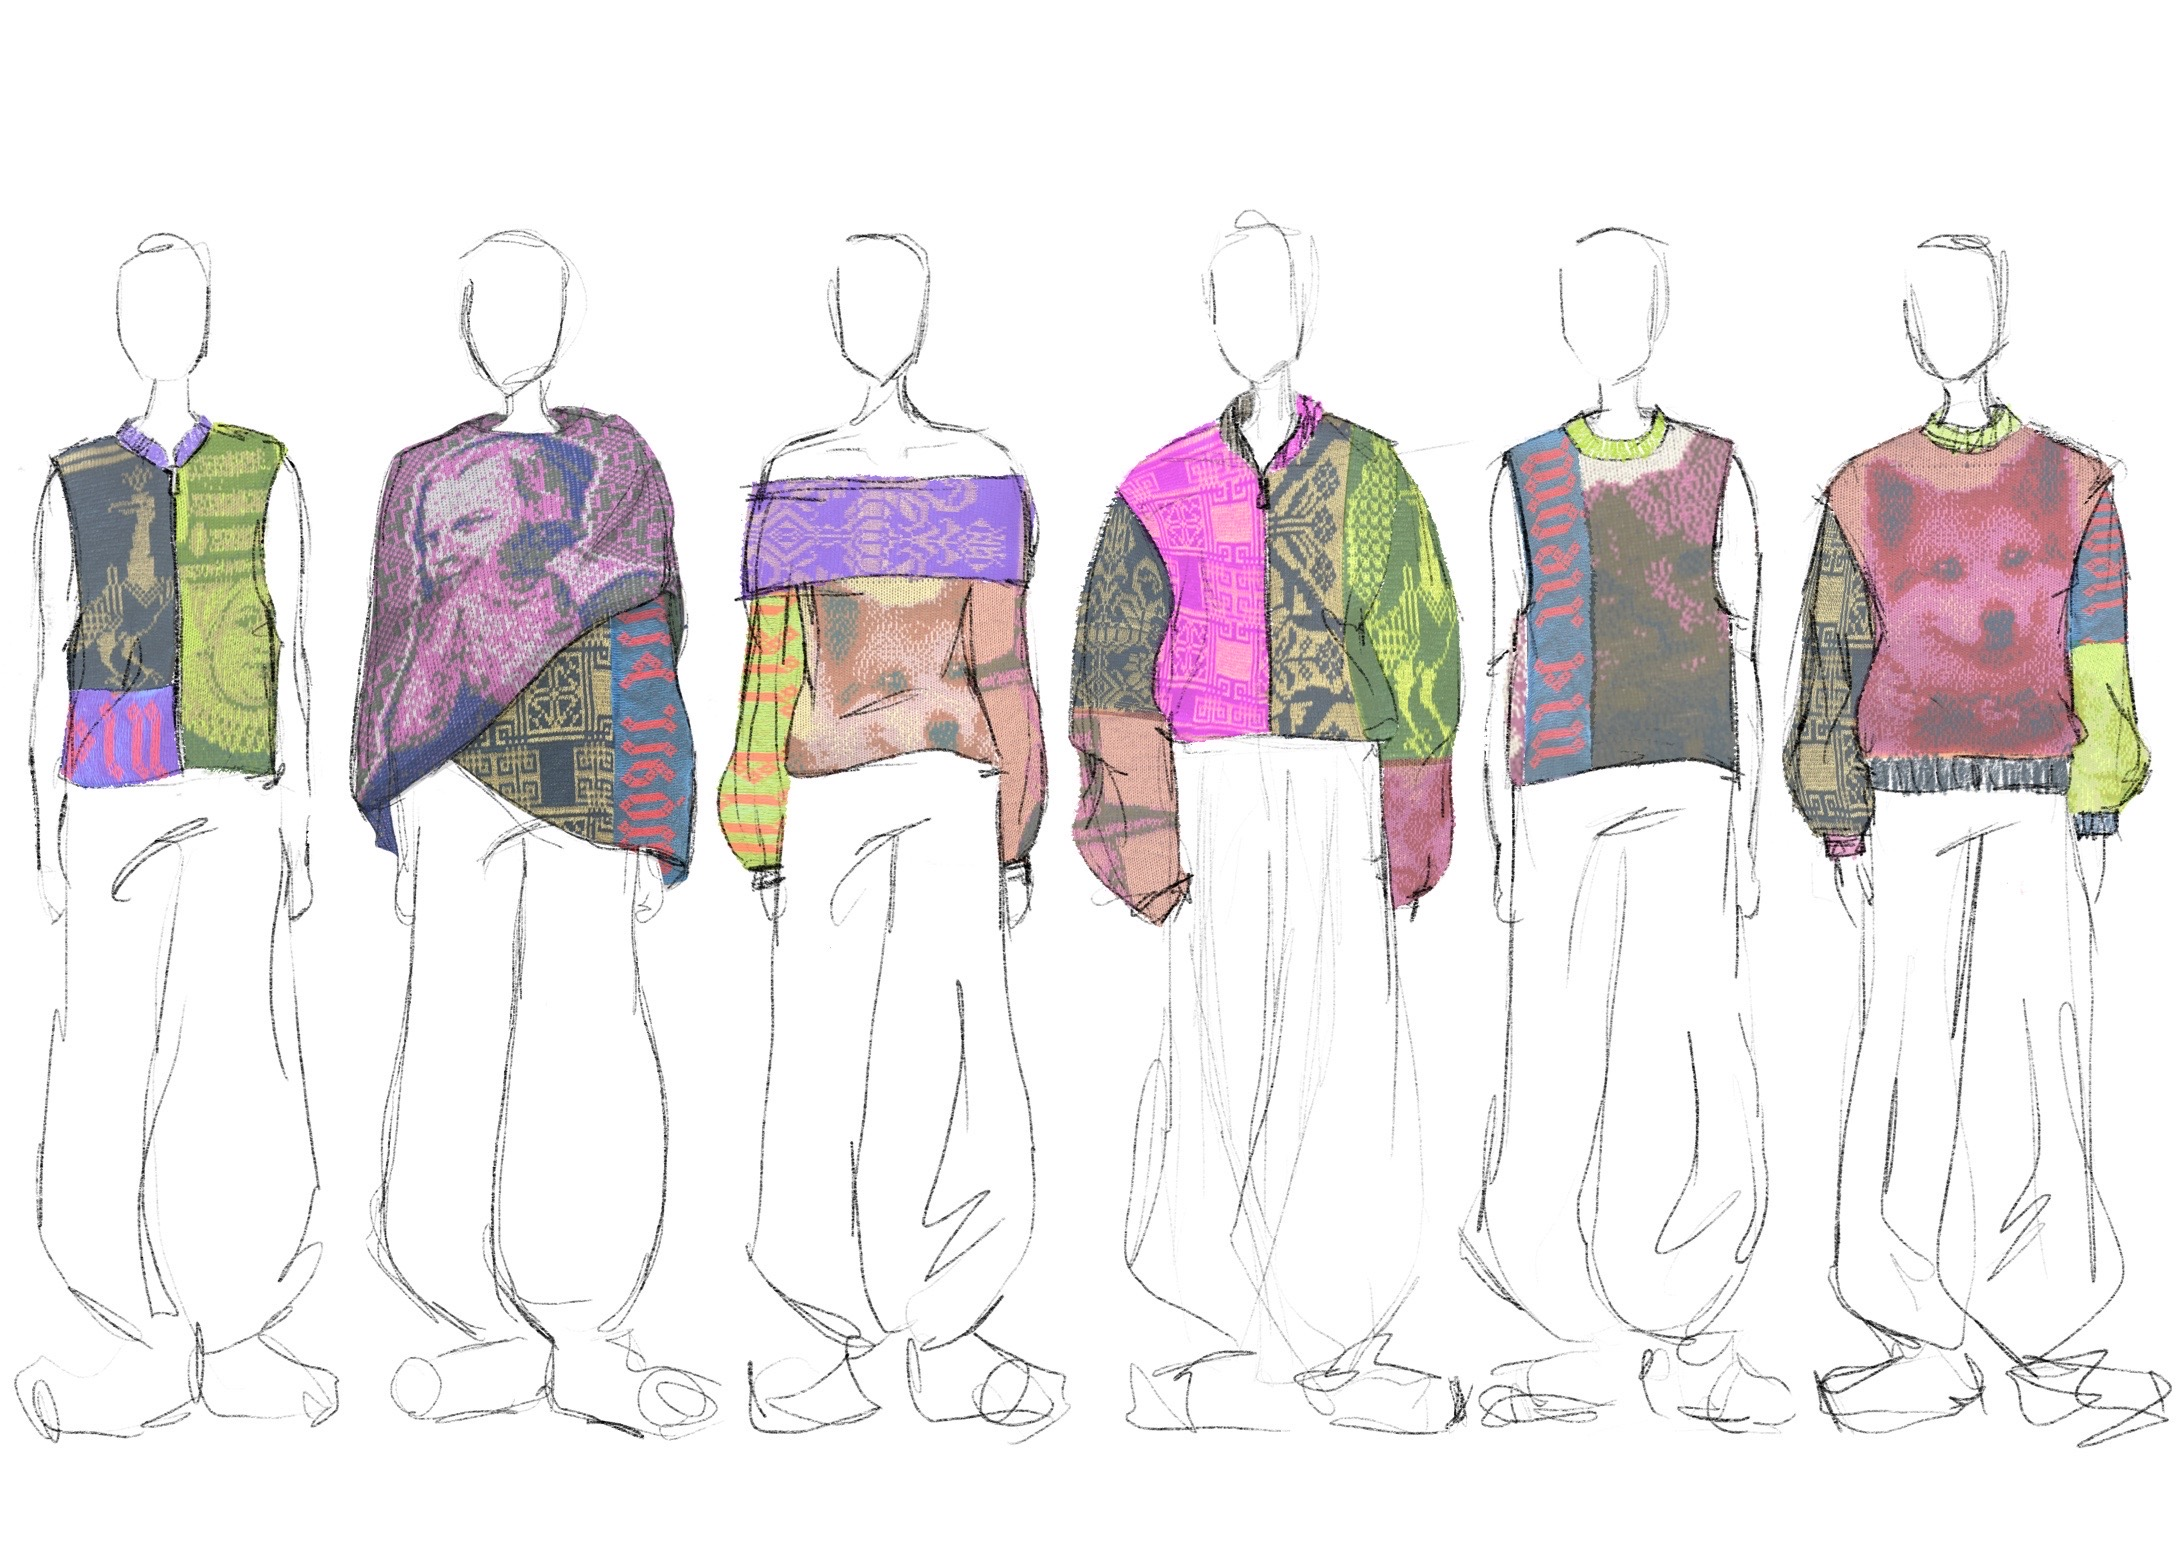
\includegraphics[width=\textwidth]{include/gisa.JPG}
\end{column}
\end{columns}
\end{frame}

{
    \usebackgroundtemplate{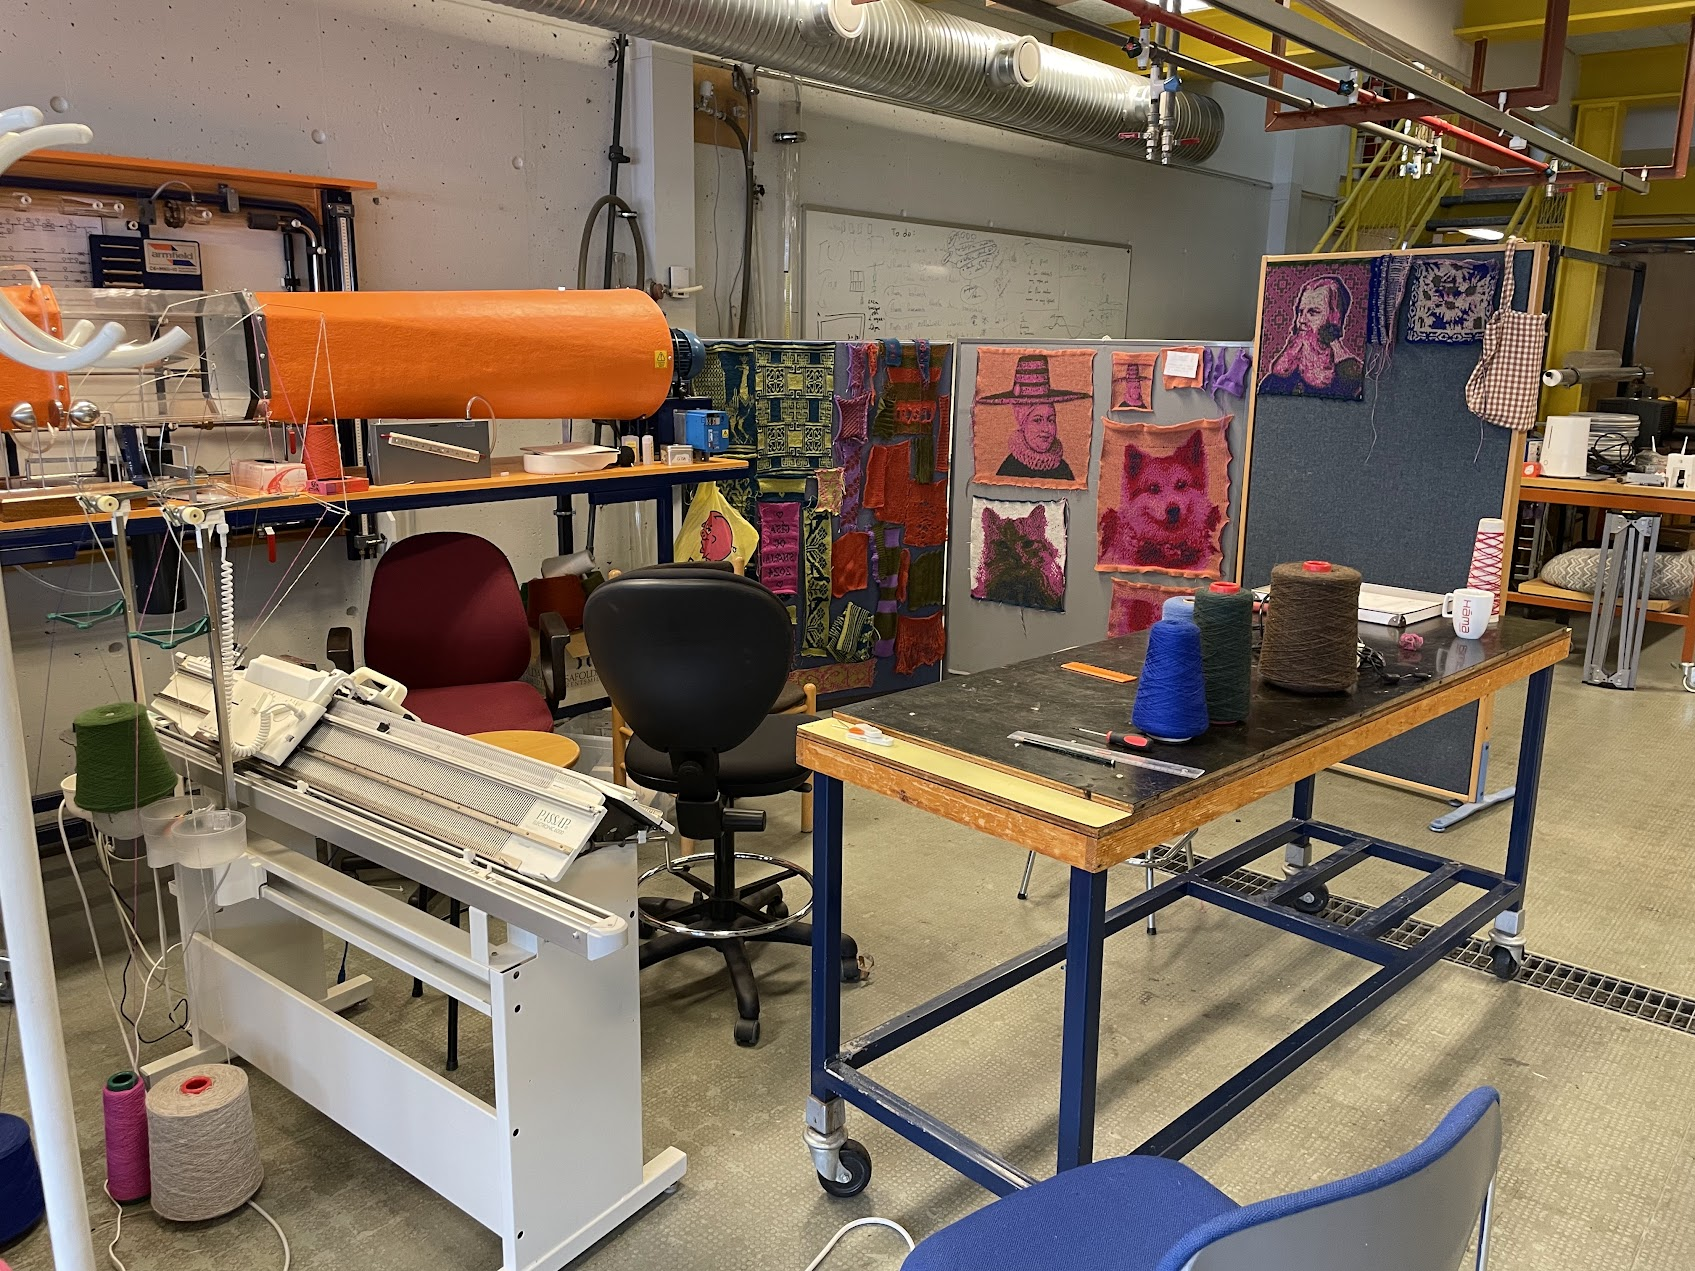
\includegraphics[width=\paperwidth]{include/workshop.jpg}}
    \begin{frame}
        \frametitle{Get in Touch}
        \vspace{2cm}
        \begin{columns}
            \begin{column}{0.4\textwidth}
            \end{column}
            \begin{column}{0.6\textwidth}
                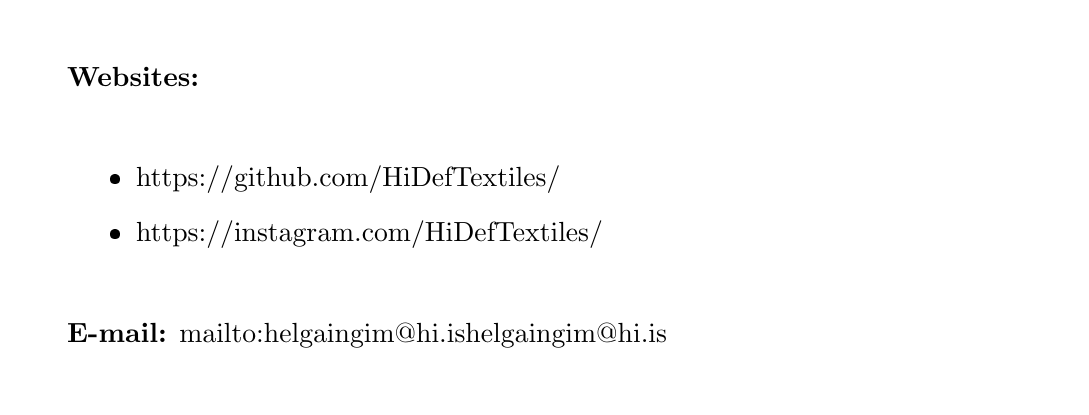
\begin{tikzpicture}
                    \node[fill=white, fill opacity=0.8, text opacity=1, inner sep=5mm] (box) {%
                        \begin{minipage}{\textwidth}
                            \textbf{Websites:}

                            \vspace{0.5cm}

                            \begin{itemize}
                                \item \url{https://github.com/HiDefTextiles/}
                                \item \url{https://instagram.com/HiDefTextiles/}
                            \end{itemize}

                            \vspace{0.5cm}

                            \textbf{E-mail:} \href{mailto:helgaingim@hi.is}{helgaingim@hi.is}
                        \end{minipage}
                    };
                \end{tikzpicture}
            \end{column}
        \end{columns}
    \end{frame}
}
\end{document}
